\documentclass[12pt,a4paper,openany,english]{extbook}
\usepackage[a4paper,includeheadfoot,margin=2.50cm]{geometry}
\usepackage{lscape}

\usepackage{tikz}
\usetikzlibrary{external}
\usetikzlibrary{decorations.pathmorphing}
\usetikzlibrary{shadows}

\raggedbottom

\renewcommand{\baselinestretch}{1.2}  % stretch horizontal space between everything by 20%


\usepackage[hyphens]{url} % Break line on hyphens in long urls
\usepackage{graphicx}
%\graphicspath{{images/}}
\usepackage{pdfpages}
\usepackage{enumitem}
\usepackage{float}
\usepackage{caption}
\usepackage{subcaption}
\usepackage[toc,page]{appendix}
\usepackage{fontspec}
\usepackage[T1]{fontenc}

% Don't indent table of contents, list of figures, and list of tables
\usepackage{tocloft}
\setlength{\cftsecindent}{0pt}    % Remove indent for \section in Table of Contents
\setlength{\cftsubsecindent}{0pt} % Remove indent for \subsection in Table of Contents
\setlength{\cftfigindent}{0pt}    % remove indentation from figures in List of Figures
\setlength{\cfttabindent}{0pt}    % remove indentation from tables in List of Tables

\usepackage{parskip} % Add space between two paragraphs and don't indent the first line of the paragraph

%
% UGent style guide
%
\setmainfont[
	Path=fonts/,
	BoldFont      =UGentPannoText-SemiBold.ttf,
	ItalicFont    =UGentPannoText-Normal.ttf,
	ItalicFeatures={FakeSlant=0.3},
	BoldItalicFont=UGentPannoText-SemiBold.ttf,
    BoldItalicFeatures={FakeSlant=0.3},
]{UGentPannoText-Normal.ttf}
\urlstyle{same}

\usepackage{color}
\definecolor{chaptergrey}{rgb}{0.5,0.5,0.5}
\usepackage[explicit, pagestyles]{titlesec}
\titleformat{\chapter}[display]{\bfseries}{\color{chaptergrey}\fontfamily{pbk}\fontsize{80pt}{100pt}\selectfont\thechapter}{0pt}{\Huge #1}
\titlespacing*{\chapter}{0pt}{-80pt}{30pt}


% Header showing chapter number and title and footer showing page number
\newpagestyle{fancy}{%
  \sethead{} % left
          {} % center
          {\Large\thechapter~~\chaptertitle} %right
  \setfoot{} % left
          {\thepage} % center
          {} %right
  \setheadrule{0pt}
}
\pagestyle{fancy}

% Header showing chapter title and footer showing page number
\newpagestyle{numberless}{%
  \sethead{} % left
          {} % center
          {\Large\chaptertitle} %right
  \setfoot{} % left
          {\thepage} % center
          {} %right
  \setheadrule{0pt}
}

% We use the package `minted` for modern code highlighting.
\usepackage[newfloat,chapter]{minted}
\SetupFloatingEnvironment{listing}{name=Code Fragment, listname=List of Code Fragments} 

\PassOptionsToPackage{hyphens}{url}
\usepackage{hyperref}
\usepackage{url}

\usepackage[numbers]{natbib}
\bibliographystyle{IEEEtran}
\usepackage[nottoc]{tocbibind}

\usepackage{booktabs}
\usepackage{array}
\usepackage{ragged2e}  % for '\RaggedRight' macro (allows hyphenation)
\newcolumntype{L}[1]{>{\raggedright\let\newline\\\arraybackslash\hspace{0pt}}m{#1}}
\newcolumntype{C}[1]{>{\centering\let\newline\\\arraybackslash\hspace{0pt}}m{#1}}
\newcolumntype{R}[1]{>{\raggedleft\let\newline\\\arraybackslash\hspace{0pt}}m{#1}}

\newcommand{\sectionbreak}{\phantomsection}

\usepackage[toc,acronym]{glossaries}  % for list of acronyms
\usepackage{glossaries-extra}
\makeglossaries                       % start internal list of acronyms

\title{Route planner based on open data}
\author{Tibo Vanheule}

\newacronym{pt}{PT}{Public Transport}
\newacronym{raptor}{RAPTOR}{Round-Based Public Transit Routing}
\newacronym{csa}{CSA}{Connection Scanning Algorithm}
\newacronym{gtfs}{GTFS}{General Transit Feed Specification}
\newacronym{netex}{NeTEx}{Network Timetable Exchange}
\newacronym{shacl}{SHACL}{Shapes Constraint Language}
\newacronym{jsonld}{JSON-LD}{JavaScript Object Notation for Linked Data}
\newacronym{rdf}{RDF}{Resource Description Framework}
\newacronym{rml}{RML}{Resource Mapping Language}
\newacronym{oslo}{OSLO}{Open standard For Linking Organisations}
\newacronym{cen}{CEN}{Comité Européen de Normalisation, European Committee for Standardization }
\newacronym{w3c}{W3C}{World Wide Web Consortium}
\newacronym{turtle}{Turtle}{Terse RDF Triple Language}
\newacronym{iri}{IRI}{Internationalized Resource Identifier}
\newacronym{nmbs}{NMBS}{Nationale Maatschappij der Belgische Spoorwegen}
\newacronym{json}{JSON}{JavaScript Object Notation}
\newacronym{csv}{CSV}{Comma Separated Values}
\newacronym{eat}{EAT}{Earliest Arrival Time}
\newacronym{meat}{MEAT}{Mininum Expected Arrival Time}
\newacronym{mc}{MC}{Multi-criteria}
\newacronym{uml}{UML}{Unified Modeling Language}
\newacronym{stib}{STIB/MIVB}{Société des Transports Intercommunaux de Bruxelles/Maatschappij voor het Intercommunaal Vervoer te Brussel}
\newacronym{ifopt}{IFOPT}{Identification of Fixed Objects in Public Transport}
\newacronym{epip}{EPIP}{European Passenger Information Profile}
\newacronym{wkt}{WKT}{Well-known text representation of geometry}
\newacronym{geojson}{GeoJSON}{Geospatial JavaScript Object Notation }
\newacronym{gis}{GIS}{Geographic information system}
\newacronym{ietf}{IETF}{Internet Engineering Task Force}
\newacronym{BSON}{BSON}{binary encoded Javascript Object Notation}
\newacronym{js}{JS}{JavaScript}
\newacronym{xml}{XML}{Extensible Markup Language}
\newacronym{http}{HTTP}{Hyper Text Transfer Protocol}
\newacronym{ptqs}{PTQS}{Public Transport Query system}
\newacronym{naptan}{NaPTAN}{National Public Transport Access Node}
\newacronym{tpeg}{TPEG}{Transport Protocol Expert Group}
\newacronym{siri}{SIRI}{Service Interface for Real Time Information}
\newacronym{api}{API}{Application Programming Interface}
\begin{document}
\frontmatter
\pagestyle{empty}

%cover sheet

\includepdf{titel-96657535.pdf}

\chapter*{Dankwoord}

Vul aan...
\chapter*{Toelichting in verband met het masterproefwerk}

Deze masterproef vormt een onderdeel van een examen. Eventuele opmerkingen die door de beoordelingscommissie tijdens de mondelinge uiteenzetting van de masterproef werden geformuleerd, werden niet verwerkt in deze tekst.

% This master's dissertation is part of an exam. Any comments formulated by the assessment committee during the oral presentation of the master's dissertation are not included in this text.

\subsection*{Melding van vertrouwelijkheid (enkel indien van toepassing)}

Bekijk hiervoor de informatie op \href{https://www.ugent.be/ea/nl/faculteit/studentenadministratie/masterproef/} {de facultaire website} - \textbf{Nota in verband met de vorm van de masterproef (alle opleidingen)}
\chapter*{Abstract}
\chaptermark{Abstract}
\addcontentsline{toc}{chapter}{Abstract}  

Meer informatie op \href{https://masterproef.tiwi.ugent.be/verplichte-taken/}{https://masterproef.tiwi.ugent.be/verplichte-taken/} - Korte abstract (Nederlands en/of Engels)

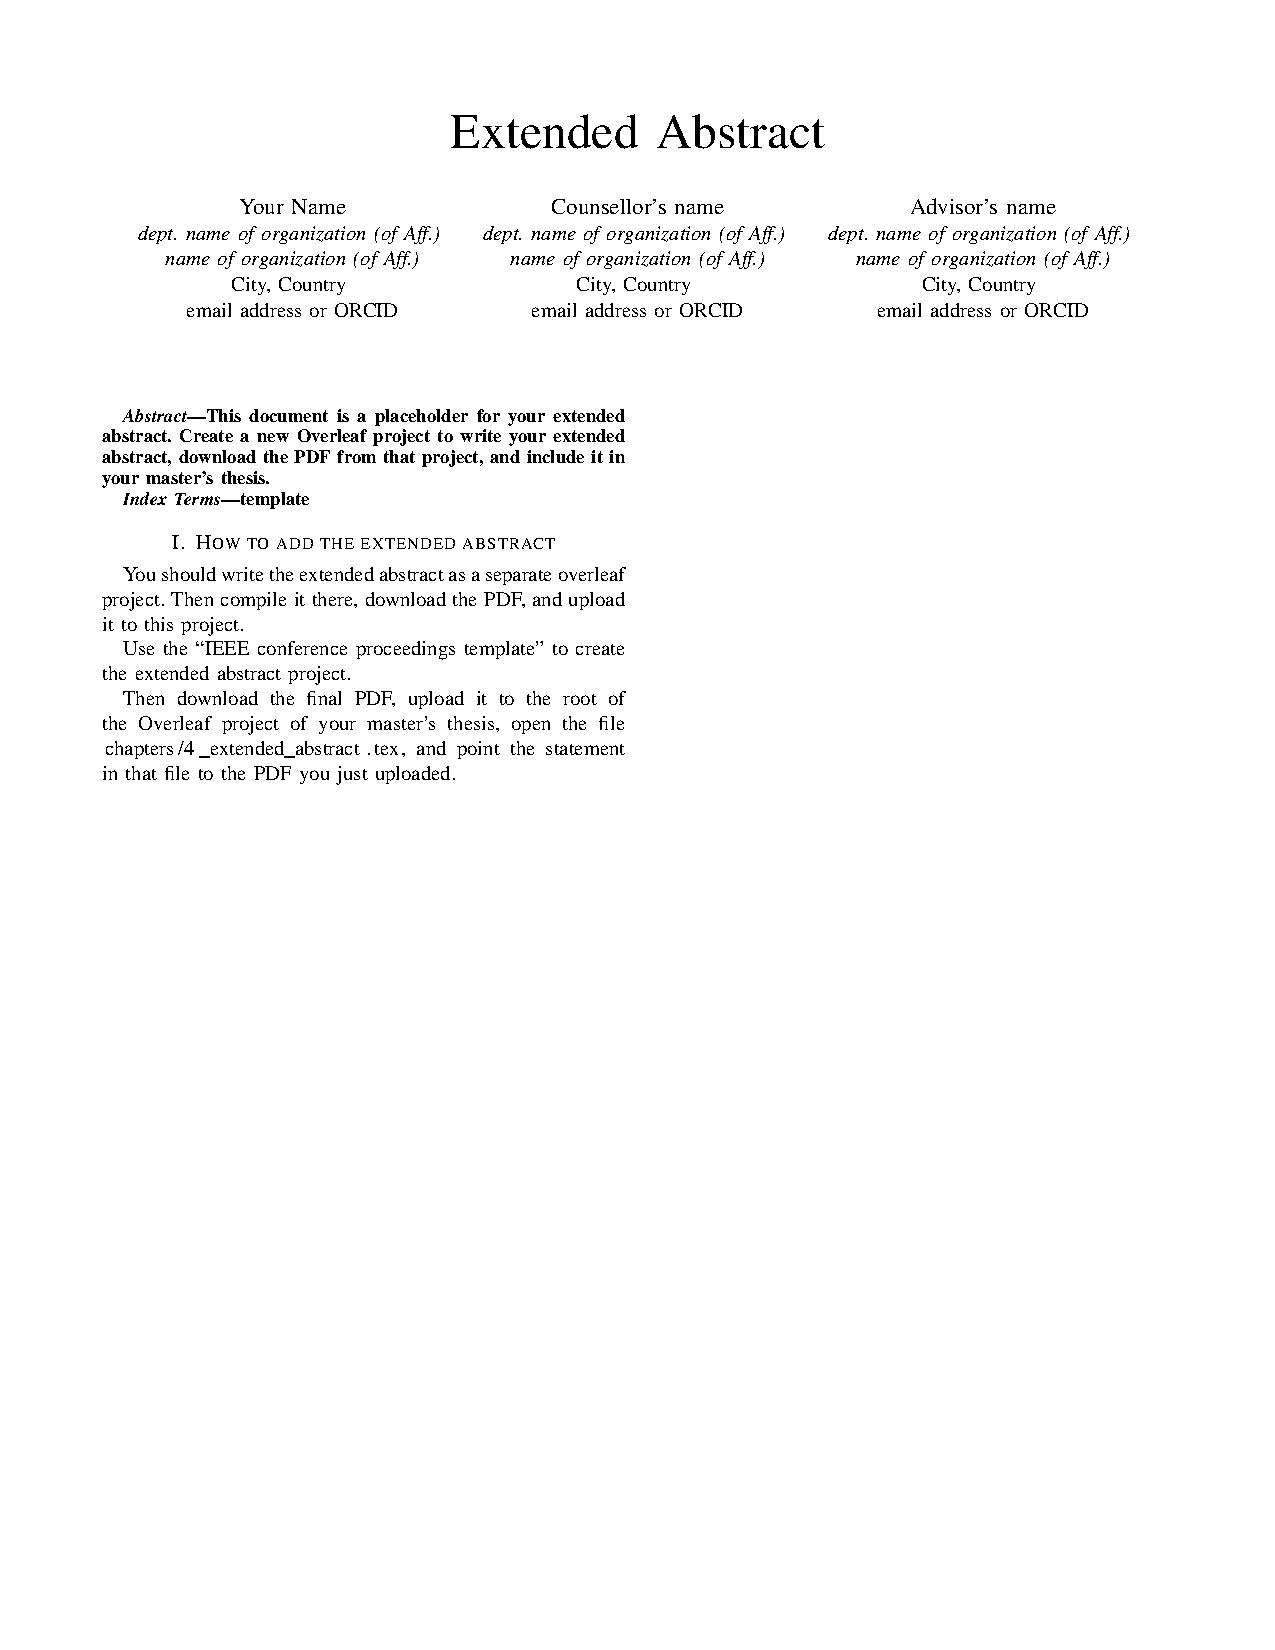
\includepdf[pages={-}]{extended-abstract.pdf}
\tableofcontents\newpage
\listoffigures\newpage
\listoftables\newpage
%%%%%%%%%%%%%%%%%%%%%%%%%%%%%%%%%%%%%%%%%%%%%%%%%%%%%%%%%%%%%%%
%                                                             %
% Note: To add or remove acronyms, modify `personal_data.tex` %
%                                                             %
%%%%%%%%%%%%%%%%%%%%%%%%%%%%%%%%%%%%%%%%%%%%%%%%%%%%%%%%%%%%%%%


% Print the glossary
\printglossary[type=\acronymtype, title={Lijst van afkortingen}]
%\printglossary[type=\acronymtype, title={List of Acronyms}] % English

\glsaddallunused[\acronymtype]                              % make sure all unused acronyms are in list

\setlist[description]{style=standard} % reset list settings back to default
\listoflistings\newpage

\mainmatter
\pagestyle{fancy}
\chapter{Introduction}
\label{chap:intro}
% bit informal introduction
Assume you are in your first year at the Belgium University of Ghent. Like most university students, you live in a dorm, and unless you lived in Ghent before moving, you do not know your way in Ghent. What is the best restaurant, and what can you do for fun? But at some point, you must go to your course, take an exam, or take a break from student life at your parents' home. Being late is not an option in these situations. But as a freshman and carless, you wonder how you will reach these destinations.  

The most obvious would be \glsxtrfull{pt}. Using \glsxtrshort{pt} is economical as a car costs ten times more yearly. Further, it is one of the few transportation modes that is environmentally friendly.

Now that you know how to reach those destinations, you wonder which route is best. Additionally, you want to be sure that you will arrive on time and at which time you should leave. 
% Intro route planners
For this last problem, there is a high chance that you will use a route planner. Many route planners exist, such as \url{nmbs.be}, \url{delijn.be} or \url{maps.google.com}. Even open-source solutions exist, like Open Trip Planner\cite{noauthor_otp_2023}.

Underlying these route planners, an algorithm calculates the "best" route serving your search criteria. They produce Pareto-optimal journeys. A journey is defined as a sequence of trips between two points. A trip can be made using a variety of transport modes (train, bus, etc.) or even on foot. One thing to remark is that if a journey contains $K$ trips, they are $K-1$ transfers. 

Commonly, these algorithms are graph-based. Although there are known speedup techniques on route planners, these speedups are generally more focused on road networks \cite{bast_car_2009}. When looking at a more specific domain, like \glsxtrshort{pt}. A few difficulties arise.

% difficulties road planners and PT
To start, \glsxtrshort{pt} has a different structure than for road networks. For example, the travel times are enough as criteria to compute a road journey, but for \glsxtrshort{pt}, additional criteria could be the number of transfers or the cost of the different transportation modes (train, bus, metro,...). These extra criteria add more complexity to the calculations.

Footpaths significantly influence the resulting Pareto journeys. It could be more efficient to walk to a different bus stop. However, unrestricted footpaths would cause too many edges in graph-based algorithms.

% centralized data strategy
Another difficulty is the centralized data strategy used by most route planners \cite{rojas_melendez_julian_andres_decentralized_2020}:
\begin{enumerate}
    \item For each transit mode, collect a dataset. A widely used format for exchanging a PT dataset is GTFS \cite{noauthor_gtfs_2022}.
    \item Integrate the collected datasets using a predefined data model in a centralized data store.
    \item Calculates available routes using a route planning algorithm tailored to run over the predefined data model.
\end{enumerate}
% problems of centralized strategy
The centralized strategy causes applications to be unscalable and results in high computational infrastructure costs (total cost of ownership). 

% work in progress
Another problem is that users cannot use the dataset in their queries if the central system does not support a third-party dataset. The data needs to be homogenous to integrate it into the route planner. If the dataset is heterogeneous, integration is done manually, and the route planner algorithm must be adapted]


\begin{figure}[H]
\centering
\resizebox{\textwidth}{!}{
\begin{tikzpicture}

\draw [stealth-stealth](0,0) -- (10,0);

\draw (10,0) node[above=32pt,right=-2.5 cm] {2013: Connection Scan Algorithm};

\end{tikzpicture}}
    \caption{This figure represents what we want to accomplish a solution that not only runs on the client and not only on the server.}
    \label{fig:shared}
\end{figure}

We want to avoid the central data strategy and let the client calculate the ideal route. However, we do not want to create a fully offline device since data will quickly become outdated and unusable. Data must be sent to the client from the server, ideally with little or no processing. 

An extra challenge is to decide which data is relevant for the client to send before the client needs it to save bandwidth and keep the number of requests low. If we send too much data, the client can become slow to high load on received.
 
Goals:
\begin{enumerate}
    \item Create a shared responsibility: The client calculates, and the server manages data.
    \item Experiment with a fragmentation to only send the required data to the client.
    \item Use an ontology to support multiple datasets/sources.
\end{enumerate}



\chapter{Related work}
\label{chap:rel_work}
%TODO When done, fix this
In this chapter we discuss the relevant literature and state of the art for this thesis, the literature is grouped in x groups. In \autoref{section:routing_rel_work}, the routing algorithms for transport are discussed. Next, we discuss the data models used in public transport, either by law or popularity (\autoref{section:data_model_rel_work}). Further, we look at developed ontologies for transportation in \autoref{section:ontologies_rel_work}.

\section{Transport Routing Algorithms }\label{section:routing_rel_work}
% include timeline image

\begin{figure}[H]
\resizebox{\textwidth}{!}{%
    \begin{tikzpicture}
    % Draw a horizontal line
    \draw (0,0) -- (4,0);
    \draw (6,0) -- (11,0);
    \draw (13,0) -- (23,0);
    
    % draw vertical lines
    \foreach \x in {0,4,6,11,13,18,23,15,20}
    \draw (\x cm,5pt) -- (\x cm,-5pt);
    
    \foreach \x in {1,8,13,21}
    \draw[line width=0.5mm, red, opacity=0.4 ] (\x cm,20pt) -- (\x cm,0);
    
    \foreach \x in {3}
    \draw[line width=0.5mm, red, opacity=0.4 ] (\x cm,0) -- (\x cm,-20pt);
    
    % draw nodes to add events
    \draw (0,0) node[below=3pt] {1955};
    \draw (4,0) node[below=3pt] {1960};
    \draw (6,0) node[below=3pt] {1985};
    \draw (11,0) node[below=3pt] {1990};
    \draw (13,0) node[below=3pt] {2005};
    \draw (15,0) node[below=3pt] {2007};
    \draw (18,0) node[below=3pt] {2010};
    \draw (20,0) node[below=3pt] {2012};
    \draw (23,0) node[below=3pt] {2015};
    
    \draw (1,0) node[above=25pt] {1956: Bellman-Ford};
    
    \draw (3,0) node[below=25pt, align=center] {1958: Dijkstra’s algorithm\\ $O(n^2)$};
    
    \draw (8,0) node[above=25pt, align=center] {1987: Tarjan\\ $O(n.\log{n})$};
    
    \draw (13,0) node[above=35pt] {2005: Dimacs challenge};
    
    \draw (16,0) node[above=0.2cm, align=center] {2008: Contraction \\Hierarchies};
    \draw[line width=0.5mm, red, opacity=0.4 ] (16 cm,5pt) -- (16 cm,0);
    
    \draw (17,0) node[below=1cm, align=center] {2009: Car or Public Transport\\ Two Worlds};
    \draw[line width=0.5mm, red , opacity=0.4] (17 cm,0) -- (17 cm,-0.8cm);
    
    
    \draw (18,0) node[above=1.5cm] {2010: Transfer patterns Hierarchies};
    \draw[line width=0.5mm, red , opacity=0.4] (18 cm,1.4cm) -- (18 cm,0);
    
    \draw (20,0) node[below=2cm] {2012: Delling’s Raptor};
    \draw[line width=0.5mm, red, opacity=0.4] (20 cm,0) -- (20 cm,-1.8cm);
    
    \draw (21,0) node[above=32pt,right=-2.5 cm] {2013: Connection Scan Algorithm};

    \draw (23,0) node[below=32pt,right=-2.5 cm] {2015: Trip-Based Public Transit Routing};
    \draw[line width=0.5mm, red, opacity=0.4] (23 cm,0) -- (23 cm,-0.8cm);
    
    
    \draw[decoration={snake},decorate] (4,0) -- (6,0);
    \draw[decoration={snake},decorate] (11,0) -- (13,0);
    \end{tikzpicture}
    }
    \caption{Timeline describing the developments in route planning. The crossed parts represent}
    \label{fig:timeline}
\end{figure}

This section discusses the state of the art and history of public transport planning. Therefore, a tiny timeline (\autoref{fig:timeline}) was constructed to visualize some important milestones explained below. As seen in the timeline, most advances were made after 2009.

\subsection{Dijkstra}
% add some dijkstra algo workings, easy
The milestones between 1956 and 2008 did not apply to PT routing but focused on normal road networks. Among these milestones was the Dijkstra algorithm, published in 1958. This was the first big improvement but had a time complexity of $O(n^2)$. An improved version was proposed almost 30 years later, in 1987. It has a complexity of $O(n*\log(n))$ and is the version of the Dijkstra algorithm learnt at schools.% It works by initializing every node to $\infty$ except the source node, which is initialized to $0$. Then, every edge of the source node is visited. 
\subsection{Dimacs challenge}
No significant improvements for route planners were made until 2005. The road network of the US was published as part of the 9th Dimacs challenge \cite{noauthor_9th_2017}. A big deal for researchers, now they had an extensive dataset to test on. Many speedup techniques, mainly pruning techniques, were devised for the Dijkstra algorithms. But this was still inapplicable to \glsxtrshort{pt}.

\subsection{Car or Public Transport: Two Worlds}
In 2009 a paper, Car or Public Transport: Two Worlds \cite{bast_car_2009}, stated "There are two kinds of people: those who travel by car, and those who use public transport.". They argued that the worlds were different, although both problems could be represented as a directed graph. For PT, we are required to deal with timetable schedules besides this spatial information.

The article covers five big "tricks of the trade" for fast routing on transportation: Bidirectional search, exploiting hierarchy, graph contraction, goal direction and distance tables. It explains why the trick works on road networks but falls short on \glsxtrshort{pt}.

\subsubsection{Bidirectional search}
A simple approach to improve Dijkstra is to search from the source node but simultaneously do a backward search from the target node. This reduces the search space by half and can be quickly done for road networks since both nodes associated with the station are known. The idea is not very effective but is critical to implementing other speedup techniques.

For \glsxtrshort{pt} this idea adds a lot of complexity since in a time-expanded graph we know the target station but not the target node. A solution is to do a backward set of all nodes associated with the end station.
\subsubsection{Exploiting hierarchy}
Roads have different levels of importance, think of motorways, national highways and minor roads. The simple routing heuristic exploits this hierarchy. When we are within a certain distance of the target and source node, we take all streets into account. In the other case, we use only high-level roads, reducing the total explored nodes. This comes with some loss of exactness.

However, this technique can be even slower in large municipal areas because the hierarchy is absent. The tram, metro and bus are equally important. A hierarchy begins to appear only when travelling long distances between cities. 
\subsubsection{Graph contraction}
\subsubsection{Goal direction}
\subsubsection{Distance tables}


This overview article marked the beginning of new PT route planners in the same ballpark as road networks regarding query speed. 
\subsection{Transfer patterns}
Transfer patterns are considered the first algorithm for PT that solves queries in an order of a few milliseconds and on a transport network with a poor structure. 

Transfer patterns describe a method using a journey planning algorithm to pre-calculate all the unique journeys for the entire graph \cite{bast_fast_2010} %wrong explanation of transfer graphs TODO FIX
. This means we can look up the schedule matching that journey when a real-time query comes in. In this case, the server can give fast query responses, but the pre-calculations can cause a computational burden. For example, the authors used a cluster of Opteron and Xeon-based 64-bit servers for their CPP implementation. Although the exact number of compute nodes is not mentioned in the paper \cite{bast_fast_2010}. 


% TODO uitleggen transfer paterns
A simple algorithm for transfer patterns illustrates the key ideas and consists of 3 parts but has quadratic precomputation complexity. A more optimized algorithm is described in the paper \cite{bast_fast_2010}.
\subsubsection{Graph}
The algorithm works on a time-expanded graph with three kinds of nodes: a departure node, an arrival node and a transfer node. Each node carries the time and the station it belongs to. Like in \autoref{fig:transferel}, an elementary connection can be formed.
\begin{figure}[H]
\begin{minipage}{.45\textwidth}

\centering
\resizebox{0.5\linewidth}{!}{%
    \begin{tikzpicture}[
roundnode/.style={circle, draw=green!60, fill=green!5, very thick, minimum size=8mm},
]
    
    \draw (0,0) -- (4,0);
    
    \draw (4,0) node[align=center,roundnode] {$Ba@t_2$};

    \draw (0,0) node[align=center,roundnode] {$Ad@t_1$};
    
    \end{tikzpicture}
%
}%
    \caption{An elementary connection betweens stations A and B, d stands for departure and a for arrival, $@t_i$ denotes the time the vehicle departs, arrives are waits (transfer)}
    \label{fig:transferel}

\end{minipage}\hspace{.1\textwidth}
\begin{minipage}{.45\textwidth}
\centering
\resizebox{0.5\linewidth}{!}{%
    \begin{tikzpicture}[
roundnode/.style={circle, draw=green!60, fill=green!5, very thick, minimum size=8mm},
]
    
    \draw (0,0) -- (4,0);
    \draw (0,0) -- (2,-2);
    \draw (0,0) -- (1,-4);
    \draw (1,-4) -- (5,-4);
    \draw (2,-2) -- (6,-2);
    
    \draw (0,0) node[align=center,roundnode] {$Bt@t_1$};

    \draw (4,0) node[align=center,roundnode] {$Bd@t_1$};


    
    \draw (2,-2) node[align=center,roundnode] {$Bt@t_2$};

    \draw (6,-2) node[align=center,roundnode] {$Bd@t_2$};

    \draw (1,-4) node[align=center,roundnode] {$Bt@t_3$};

    \draw (5,-4) node[align=center,roundnode] {$Bd@t_3$};
    \end{tikzpicture}
%
}%
    \caption{An transfer, with an waiting chain}
    \label{fig:transferpatterntransfer}

\end{minipage}
\end{figure}
\subsubsection{Fast direct-connections queries}
This part is only for direct connections, meaning a maximal path in the graph without transfer nodes.

\begin{enumerate}
    \item Precompute all maximal paths in the graph without transfer nodes. Group them in lines that share the same sequence of stations. This creates an ordered timetable for a particular line.
    \item Precompute for each station the sorted list of lines in which the station occurs and its position(s) on the line. This creates a lookup table, which can be used to find timetables of lines stations share.
    \item To answer a direct connection query, use the precomputed sorted list of the departure and arrival stations. See if they share a line with the departure station, which has a lower position than the arrival station. Using the timetables of the found lines, determine the earliest arrival time.
\end{enumerate}
\subsubsection{Transfer patterns precomputation}
\subsubsection{Query graph construction and evaluation}
\subsubsection{scalable transfer patterns}
% IDEA, HYDRIDE? 
\subsection{\glsfmtfull{csa}}
\subsection{\glsfmtfull{raptor}}
RAPTOR is a graph-based algorithm which solves queries in rounds. Round K computes the fastest way of getting to every stop with at most k - 1 transfers or k trips.

\begin{enumerate}
    \item Each node gets a multilabel. $(\tau_0,...,\tau_k)$ with $\tau_i$ representing the earliest arrival time in $i$ trips. We init all arrival times in each label with $\infty$. Except for the departing node, where $\tau_0$ is set to the depart time of our search criteria.
    \item For each round $k$ our goal is to compute $\tau_k$. This happens in three stages:\begin{enumerate}
        \item Set the earliest arrival time k ($\tau_k$) to that of iets predescor ($\tau_{k-1}$). This is an upper bound since we are not interested in slower stop times than the previous round.
        \item We iterate over the routes. We calculate the earliest trip we can take for each stop $p$ on the route $r$. This does not always exist. We search stops along the route $r$ with the earliest trip $t$. This means we can hop on the route $r'$ in $p$. For subsequent stops in $r'$, we can update $\tau_k$ according to the found trip $t$.
        \item Finally, footpaths are considered. We check if $\tau_k$ can be improved by using a footpath between two stops. 
    \end{enumerate}
\end{enumerate}


\begin{figure}[H]
\centering
\resizebox{\textwidth}{!}{%
    \begin{tikzpicture}[
roundnode/.style={circle, thick, minimum size=7mm, text width=3.5cm,align = center,scale=0.6,font=\huge},
green/.style={draw=green!60, fill=green!5},
orange/.style={draw=orange!60, fill=orange!5},
white/.style={draw=black!60, fill=white},
]
    \draw (0.4,-2) node[right=0] {Legend:};
    \draw [dashed](2,-2) -- (2.5,-2);
    \draw (2.6,-2) node[right=0] {= unprocessed,};
    \draw [](5,-2) -- (5.5,-2);
    \draw (5.6,-2) node[right=0] {= processed,};
    \draw (7.8,-2) node[roundnode,text width=0.4cm,green,right=0] {};
    \draw (8.2,-2) node[right=0] {= source,};
    \draw (10,-2) node[roundnode,text width=0.4cm,orange,right=0] {};
    \draw (10.4,-2) node[right=0] {= target.};
    
    \draw [dashed](0,0) -- (6,0);
    \draw [](9,0) -- (15,0);
    \draw [](18,0) -- (24,0);
    

    \draw [dashed](6,0) -- (6,5);
    \draw [dashed](15,0) -- (15,5);
    \draw [](24,0) -- (24,5);
    

    \draw [dashed](0,0) -- (6,5);
    \draw [](9,0) -- (15,5);
    \draw [](18,0) -- (24,5);
    
    \draw[->, ultra thick] (7,2.5) -- (8,2.5);
    \draw[->, ultra thick] (16,2.5) -- (17,2.5);
    
    \draw (0,0) node[roundnode,green] {9:00,$\infty$};
    \draw (3,0) node[roundnode,white] {$\infty,\infty$};
    \draw (6,0) node[roundnode,white] {$\infty,\infty$};
    \draw (3,2.5) node[roundnode,white] {$\infty,\infty$};
    \draw (6,5) node[roundnode,orange] {$\infty,\infty$};

    
    \draw (9,0) node[roundnode,green] {9:00,$\infty$};
    \draw (12,0) node[roundnode,white] {9:30,$\infty$};
    \draw (15,0) node[roundnode,white] {10:00,$\infty$};
    \draw (12,2.5) node[roundnode,white] {11:00,$\infty$};
    \draw (15,5) node[roundnode,orange] {11:30,$\infty$};

    
    \draw (18,0) node[roundnode,green] {9:00,9:00};
    \draw (21,0) node[roundnode,white] {9:30,9:30};
    \draw (24,0) node[roundnode,white] {10:00,10:00};
    \draw (21,2.5) node[roundnode,white] {11:00,11:00};
    \draw (24,5) node[roundnode,orange] {11:30,10:30};

    \draw (2.5,7) node[font=\Large] {initialization};
    \draw (12,7) node[font=\Large] {round 1};
    \draw (21,7) node[font=\Large] {round 2};
    \end{tikzpicture}
%
}%
    \caption{A small example using raptor, two rounds are show}
    \label{fig:raptor_example}
\end{figure}

\subsubsection{Hyper partitioning}
Hyper partitioning is a preprocessing-based acceleration technique for computing bi-criteria Pareto-optimal journeys in public transit networks, based on the well-known RAPTOR algorithm \cite{delling_round-based_2015}.
\subsubsection{unrestricted footprints}
\section{Data Models For public transport}\label{section:data_model_rel_work}
\subsection{What is a data model }
% TODO CHECK AND REWRITE 
% FROM https://cedar.princeton.edu/understanding-data/what-data-model
A data model organizes data elements and standardizes how the data elements relate to one another. Since data elements document real-life people, places and things and the events between them, the data model represents reality. For example, a house has many windows, or a cat has two eyes.

Data models are often used as an aid to communication between the business people defining the requirements for a computer system and the technical people defining the design in response to those requirements. They are used to show the data needed and created by business processes.
 
A data model explicitly determines the structure of data. Data models are specified in a data modelling notation, which is often graphical in form.]
A data model can be sometimes referred to as a data structure, especially in the context of programming languages. Data models are often complemented by function models.
\subsection{\glsfmtfull{gtfs}}
\glsfmtfull{gtfs} defines a common format for public transportation schedules and associated geographic information. "feeds" let public transit agencies publish their transit data. The developer can then write applications.
\subsubsection{\glsfmtshort{gtfs} feed}
A feed is a zip file that contains CSV files but typically uses the .txt extension. Some essential files include stops.txt, routes.txt and trips.txt.


\subsection{\glsfmtfull{netex}}
The NeTEx defines a standard for exchanging public transport passenger information data in XML format. The functional
scope of NeTEx is divided into three parts, each covering a functional subset of the CEN Transmodel conceptual
model for Public Transport Information, [T1], [T2], [T3].
Part 1 [N1]] describes the fixed Network (stops, routes, lines, etc.); Part 2 [N2] is mainly focused on Timetables and
Part 3 [N3] covers Fare data (and is the main subject of this paper). All three parts use the same framework of reusable
components, versioning mechanism, validity conditions, and support to allow the unique identification of data elements
in a global context, etc., defined in Part 1. NeTEx also includes container elements called "VERSION FRAMES"
to group data into coherent sets for efficient exchange.
NeTEx deliverables comprise (i) a CEN Specification document (in three parts), (ii) a data model in the standard UML
modelling language [U1] and (iii) an accompanying XML schema providing a formal electronic description that can
be used by data processing software.

Data in NeTEx format is encoded as XML documents that must conform exactly to the schema – standard XML validator tools can check conformance automatically. The schema can also be used to create bindings for different
programming languages, automating part of the implementation process for creating software that supports NeTEx
formats. 
\subsubsection{NETEX profiles}
\subsection{Transmodel}
\section{Semantic Web and the role of Ontologies}\label{section:ontologies_rel_work}
\subsection{Semantic Web}
The semantic web can be seen as an extension of the current web and is a vision of Tim Berners-Lee, where web documents not only describe how to render data visually. The data is also annotated with terms to express how it should be interpreted. So, web documents also capture the meaning of the information.
\subsection{Resource Description Framework}
\subsection{JSON-LD}
%\subsection{RML}

\subsection{Ontologies}
The best definition of an ontology states: "An ontology is an explicit specification of a conceptualization" \cite{gruber_translation_1993}. Many ontologies exist, from basic to formal ontologies specified in highly expressive logic. In this thesis, we mainly use formal ontologies.

These ontologies play an essential role in the semantic web. 

A small study was conducted to find an ontology that best suited our needs. Many of the studied ontologies for transport are focused on specific use cases, for example, urban freight \cite{bouhana_ontology-based_2015}. They do not have a broad domain. 
\subsection{x}
A relatively old ontology designed to use with a user planning tool based on journey patterns \cite{5507372} was found and could support RAPTOR. Interestingly, they implemented a mobile application to plan tourist bus routes, but it relied on server-side queries. Other downsides are that there is no multi-modal support (only transport by bus) and no multi-operator support. The ontology was not directly available from the authors.

Using the survey of transportation ontologies \cite{katsumi_ontologies_2018}, we only identify three ontologies that support journey patterns. Two are focused on city logistics and urban systems, which are different domains. The last ontology (Transportation ontology for content personalization) applies to PT, but the ontology is not directly available.

\subsection{Transmodel ontology}
European directives require every PT agent to be compatible with Transmodel, so an ontology aligned with Transmodel is interesting. Further, the Transmodel ontology supports journey patterns. However, the ontology could be too broad, which leads to several potential problems. For example, it can make it hard to find relevant information, as the ontology may contain too many concepts and relationships that are not relevant. Furthermore, as the ontology may not be compatible with other ontologies used in those sources, integration from different sources can also be challenging.

\subsection{OSLO Mobiliteit: Dienstregeling en Planning}
The last ontology we looked at is the "OSLO Mobiliteit - Dienstregeling en Planning" \cite{noauthor_oslo_2023} ontology. The ontology is developed by Open Standaarden voor Linkende Organisaties (OSLO), a department of Data Flanders. It has been based on the EPIP profile of NETEX. NETEX is based directly on  Transmodel, so the ontology has some similarities with the Transmodel ontology but is less broad than the Transmodel ontology.

\begin{landscape}
\begin{table}[]
\centering
\begin{tabular}{|l|l|l|l|l|l|l|}
\hline
\textbf{Ontology} &
  \textbf{\begin{tabular}[c]{@{}l@{}}Journey\\ patterns?\end{tabular}} &
  \textbf{\begin{tabular}[c]{@{}l@{}}Multi-\\ modal?\end{tabular}} &
  \textbf{\begin{tabular}[c]{@{}l@{}}Multi-\\ operator?\end{tabular}} &
  \textbf{\begin{tabular}[c]{@{}l@{}}Designed for use\\  with routeplanners\end{tabular}} &
  \textbf{\begin{tabular}[c]{@{}l@{}}directly available\\  for reuse?\end{tabular}} &
  \textbf{DOI} \\ \hline
\begin{tabular}[c]{@{}l@{}}Intoducing the public transport\\ domain to the web of data\end{tabular} &
  yes &
  yes &
  yes &
  yes &
  no &
  10.1007/978-3-319-11746-1\_38a \\ \hline
iCity Ontology &
  yes &
  no &
  no &
  no, urban systems &
  yes, GitHub &
  w3id.org/icity/iCityOntology\_v1\_Report.pdf \\ \hline
Genclon &
  yes &
  no &
  no &
  no, city logistics &
  no &
  10.1016/j.eswa.2012.03.068 \\ \hline
\begin{tabular}[c]{@{}l@{}}Transportation ontology\\ for content personalization\end{tabular} &
  yes &
  yes &
  yes &
  yes &
  no &
  10.1016/j.eswa.2012.12.028 \\ \hline
Transmodel ontology &
  yes &
  yes &
  yes &
  yes &
  yes, GitHub &
  10.3233/SW-210451 \\ \hline
OSLO Ontology &
  yes &
  yes &
  yes &
  yes &
  yes &
  / \\ \hline
\end{tabular}
\caption{}
\label{tab:my-table}
\end{table}
\end{landscape}
\chapter{Implementation}
\label{chap:implementation}

The implementation was divided into \FetchStoredCounterValue{section} parts. We discuss the implementation of \glsxtrshort{raptor} for the browser in \autoref{section:implementation_raptor}. The download of GTFS data is discussed in \autoref{section:gtfsdownloader}. The conversion of the \glsxtrshort{gtfs} data is explained in \autoref{section:implementation_data_ontology} and fragmentation in \autoref{sec:fragimpl}. Lasty, we discus what we have used for the demo in \autoref{sec:demo}


\section{\glsfmtfull{raptor} implementation}\label{section:implementation_raptor}
\subsection{Data usage of existing implementation}
Since an existing implementation of Raptor inspired us, we researched which data the implementation used.

Small description of the used text files in the \glsxtrshort{gtfs}-feed and how they are transformed.
\begin{itemize}
    \item \textbf{calendar.txt}: Used to create an Calendar Object with a "service\_id" as key
    \item \textbf{stops.txt}: to create a Stop object with key stop\_id
    \item \textbf{calendar\_dates.txt}: Creates a Dates object with key service id. Holds all key dates on which a service is active. Using exception\_type === "1" (service exceptions)
   \item \textbf{trips.txt}: Creates a huge array of trips.
   \item  \textbf{stop\_times.txt}: Used to create a list of Stoptimes with key trip\_id.
   
   \item \textbf{transfers.txt}: This creates two objects. If the transfer is from and to the same stop, we create an "interchange" object. But else we create a "transfers" object with a key "from\_stop\_id". In our feed from \glsxtrshort{nmbs}, we only got interchanges and no transfers.
\end{itemize}

\subsubsection{Not used but are in our \glsxtrshort{gtfs}-feed}
\begin{itemize}
    \item feed\_info: Information of the feed itself. The publisher is not necessarily the agency itself.
    \item agency: Information about the agency providing the services.
    \item areas: Optional file, Defines area identifiers.
    \item translations: Optional file, useful for a country with multiple languages.
\end{itemize}
\subsubsection{Unavailable in feed}
There are a lot of files that are marked as optional in the reference \cite{noauthor_gtfs_2022} that are not present in our file:
fare\_attributes.txt,
    fare\_rules.txt,
    timeframes.txt,
    fare\_media.txt,
    fare\_products.txt,
    fare\_leg\_rules.txt,
    fare\_transfer\_rules.txt,
    stop\_areas.txt,
    networks.txt,
    route\_networks.txt,
    shapes.txt,
    frequencies.txt,
    pathways.txt,
    levels.txt,
    location\_groups.txt,
    location\_group\_stops.txt,
    locations.geojson,
    booking\_rules.txt and
    attributions.txt

\subsection{Little mistakes of the implementation}
\subsubsection{unused information from gtfsfeed}
The algorithm did not use some information but was thereby inferred. For example:
\begin{itemize}
    \item Order of stop points. Each stop point in a sequence was based on its position in the array, which is not a big problem if the array is correctly sorted. But a \glsxtrshort{gtfs} feed requires each stop point to carry information like their position in the sequence. This is more correct since it supports feeds with incorrectly sorted stop points.
    \item Route id was not used but created from the trip\_id and all the stop times in that trip. Since our solution will be more dynamic and not include all stop times simultaneously, we will not follow the same structure.
\end{itemize}
\subsection{Important classes}
The \glsxtrshort{raptor} implementation is modular. These are the most important classes we will refactor in later steps:
\begin{itemize}
    \item \textbf{RaptorAlgortihmFactory}: This is a factory to create a RaptorAlgorithm instance. Before making such an instance, it indexes the data from the \glsxtrshort{gtfs}-parser.
    \item \textbf{QueueFactory}: This creates a queue on each iteration of the \glsxtrshort{raptor} algorithm.
    \item \textbf{RouteScanner}: This returns the earliest trip of a route, remembers the last trip in reference, and will not return the trip twice. This is essentially an iterator over trips in a route.
    \item \textbf{RaptorAlgorithm}: Implementation of the \glsxtrshort{raptor} algorithm, but heavily depends on de ScanResults class.
    \item \textbf{ScanResults}: Defines helper methods for the Raptor Algorithm.
\end{itemize}
\subsection{DataLoader: a new class}
The old implementation used a data flow that was unhandy for our goal. First, the RaptorAlgorithmFactory received the data that was parsed by the old parser. It then proceeded to create indexes and data structures. Then, it spreads that data to the relevant classes to create a RaptorAlgorithm.

\makeatletter
\begin{figure}[H]
\centering
\resizebox{.8\textwidth}{!}{%
    \begin{tikzpicture}[rect/.style={shape=rectangle,draw=black,semithick,align=center},
    ]
    % QueueFactory(, ),
    %       new RouteScannerFactory(tripsByRoute),

        
    % draw nodes
    \node[rect] (RaptorAlgorithmFactory) at (2,0) {RaptorAlgorithmFactory};
    \node[rect] (ScanResultsFactory) at (10,0) {ScanResultsFactory};
    \node[rect] (QueueFactory) at (7,-2) {QueueFactory};
    \node[rect] (RouteScannerFactory) at (2,-2) {RouteScannerFactory};

    \node[rect] (RaptorAlgorithm) at (2,-5) {RaptorAlgorithm};
    
    \draw (RaptorAlgorithmFactory) edge[->] node[above,pos=0.5,font=\footnotesize] {usefulTransfers} (ScanResultsFactory);

    \draw (RaptorAlgorithmFactory) edge[->] node[right,pos=0.4,font=\footnotesize] {routesAtStop} node[right,pos=0.65,font=\footnotesize] {routeStopIndex} (QueueFactory);

    \draw (RaptorAlgorithmFactory) edge[->] node[left,pos=0.5,font=\footnotesize] {tripsByRoute} (RouteScannerFactory);

    \draw (RaptorAlgorithmFactory) edge[->, bend right=80] node[left,pos=0.4,font=\footnotesize] {routeStopIndex} node[left,pos=0.5,font=\footnotesize] {routePath} node[left,pos=0.6,font=\footnotesize] {usefulTransfers} node[left,pos=0.7,font=\footnotesize] {interchange} (RaptorAlgorithm);
    
    \draw (RouteScannerFactory) edge[->,bend right=30] node[right,pos=0.5,font=\footnotesize] {RouteScannerFactory} (RaptorAlgorithm);

    \draw (QueueFactory) edge[->, bend left=15] node[right,pos=0.5,font=\footnotesize] {QueueFactory} (RaptorAlgorithm);

    \draw (ScanResultsFactory) edge[->,bend left=35] node[right,pos=0.5,font=\footnotesize] {ScanResultsFactory} (RaptorAlgorithm);
    
    \end{tikzpicture}
    }
    \caption{This represents the dataflow of the \glsxtrshort{raptor} in order to createan RaptorAlgorithm}
    \label{fig:dataflow}
\end{figure}
\makeatother

A new class, Dataloader, was created to hold all data in one class. The class will also handle all requests for new fragments and process these new fragments to populate the needed data structures.

We moved the following data holders to the DataLoader class and made them a private field. For each private field, a getter/setter is generated. This allows us to control access to these private fields.
\begin{itemize}
    \item \textbf{tripsByRoute}: This holds all the trips corresponding to a route. Primarily used by RouteScanner, which uses this to give back an interesting trip for the \glsxtrshort{raptor} algorithm.
    \item \textbf{routeStopIndex}: Contains all the corresponding stops of a route; for each stop, it stores the index in the route.\\ For example $\{route\_id\_1:\{stop\_id\_1:1,stop\_id\_2:2\}\}$.
    \item \textbf{routePath}: Contains a list of stop IDs for each route.\\ For example: $\{route\_id\_1:[stop\_id\_1,stop\_id\_2]\}$
    \item \textbf{routesAtStop}: This contains a list of all possible routes (regardless of whether a trip is running or not) possible at a given stop.
    \item \textbf{interchange}: This list defines how long a transfer in the same station takes.
    \item \textbf{usefulTransfers}: A list of transfers between nearby stations. For example, stations 100 meters away can be done by foot.
\end{itemize}

We then changed RouteScanner, RouteScannerFactory, ScanResults, ScanResultsFactory and QueueFactory to use our new class.

To the constructor of the Dataloader, we also pass the origin and destination. Then, after creation, we call the function "first". This function gets the first fragment starting from the origin. Since we had to await the request for the fragment, we could not place this in the constructor since in \glsxtrshort{js}, constructors can not be made async.

\makeatletter
\begin{figure}[H]
\centering
\resizebox{.8\textwidth}{!}{%
    \begin{tikzpicture}[rect/.style={shape=rectangle,draw=black,semithick,align=center},
    ]

    % draw nodes
    \node[rect] (RaptorAlgorithmFactory) at (2,0) {RaptorAlgorithmFactory};
    \node[rect] (ScanResultsFactory) at (10,0) {ScanResultsFactory};
    \node[rect] (QueueFactory) at (7,-2) {QueueFactory};
    \node[rect] (RouteScannerFactory) at (2,-2) {RouteScannerFactory};

    \node[rect] (RaptorAlgorithm) at (2,-5) {RaptorAlgorithm};
    
    \draw (RaptorAlgorithmFactory) edge[->] node[above,pos=0.5,font=\footnotesize] {Dataloader instance} (ScanResultsFactory);

    \draw (RaptorAlgorithmFactory) edge[->] node[right,pos=0.5,font=\footnotesize] {Dataloader instance} (QueueFactory);

    \draw (RaptorAlgorithmFactory) edge[->] node[left,pos=0.5,font=\footnotesize] {Dataloader instance} (RouteScannerFactory);

    \draw (RaptorAlgorithmFactory) edge[->, bend right=80] node[left,pos=0.5,font=\footnotesize] {Dataloader instance} (RaptorAlgorithm);
    
    \draw (RouteScannerFactory) edge[->,bend right=30] node[right,pos=0.5,font=\footnotesize] {RouteScannerFactory} (RaptorAlgorithm);

    \draw (QueueFactory) edge[->, bend left=15] node[right,pos=0.5,font=\footnotesize] {QueueFactory} (RaptorAlgorithm);

    \draw (ScanResultsFactory) edge[->,bend left=35] node[right,pos=0.5,font=\footnotesize] {ScanResultsFactory} (RaptorAlgorithm);
    
    \end{tikzpicture}
    }
    \caption{This represents the new dataflow of the \glsxtrshort{raptor} to create a RaptorAlgorithm. Note that RaptorAlgorithmFactory first creates an instance of Dataloader and shares that instance.}
    \label{fig:dataflownew}
\end{figure}
\makeatother
\subsubsection{}


\subsection{Adapt for the browser}
The browser can run compiled Typescript or JavaScript natively. Initially, t \glsxtrshort{js} applications were pretty small, but over recent years, they got bigger. This has been sped up by the introduction of Node.js, where \glsxtrshort{js} is used in a different context. 

This created a need for a way to split up \glsxtrshort{js}-applications into modules. Node.js already supports modules, but the good thing is that recently, the browser has also started to support modules. \cite{noauthor_javascript_2024}

This means we can easily import our \glsxtrshort{js} code after compiling the Typescript and then execute it in the browser.

To simplify the import, we bundle all our script files into one file using Esbuild \cite{noauthor_esbuild_nodate}. It is an extremely fast bundler that takes only 20 ms to bundle and transform our code. This is mainly because it is written in Go and compiles to native code. Further, it uses parallelisation and efficient use of memory.

This is even faster than the typical Typescript compile command $npm\ run\ tsc$!

Other handy options of the bundler are:
\begin{enumerate}
    \item \textbf{minify}: minify the code like whitespace. Reduces our code with 10 Kilobytes.
    \item \textbf{target}: Further optimisations can be unlocked with the option target. An example is \\$a === undefined || a == null? 1 : a$ could be minified to $a ?? 1$. Or, in reverse, transform \glsxtrshort{js} syntax that is too new for these environments into older JavaScript syntax that will work in these environments.
    \item \textbf{drop:console}: automatically remove all console statements.
    \item \textbf{sourcemaps}: This is essential for debugging. These maps encode the information necessary to translate from a line/column offset in a generated output file to a line/column offset in the original input file. This is very handy if TypeScript or minification is used.
\end{enumerate}

The target option is essential because it ensures that all the node-specific APIs get converted to code supported by the browser.

\begin{listing}[H]
    \begin{minted}[frame=single,linenos, breaklines]{bash}
esbuild ./queries.js --bundle --sourcemap --target='chrome124,firefox124' --format=esm --outfile=browser.js
    \end{minted}
    \caption{Command to bundle our \glsxtrshort{js} code for debugging}
\end{listing}
\begin{listing}[H]
    \begin{minted}[frame=single,linenos, breaklines]{bash}
esbuild ./queries.js --bundle --target='chrome124,firefox124' --format=esm --outfile=browser.js --minify
    \end{minted}
    \caption{Command to bundle our \glsxtrshort{js} code for production}
\end{listing}
\section{GTFS downloader}
\label{section:gtfsdownloader}
Since a GTFS feed is a zip file valid for a certain period, we need a small program to manage all these versions. This led to a Node.js module gtfs-downloader\footnote{Available as GitLab project under the same name. \\\url{https://gitlab.ilabt.imec.be/KNoWS/master-thesis/tibou-vanheule/gtfs-downloader}}. It provides the file path of the GTFS zip archive that either has been downloaded in the past or is freshly downloaded. So, it also acts like a cache and is more important than it appears, as only the most recent is available on the server. For debugging and experimenting while developing, it is handy that we have some control over the version in use. 

Two sets of functionality are represented in \autoref{fig:gtfsdownloader}. The first is when we already know the version we want to download. We search if it exists in our data folder; if not, we check if it is available on the server for download.

In the other case, we want to have the latest version, and we send a head request to the server\footnote{Server URL is specified in a dot env config} since we are only interested in the LastModified header. We check if that version is available locally; otherwise, we download the zip file.
\makeatletter
\begin{figure}[H]
\centering
\resizebox{.8\textwidth}{!}{%
    \begin{tikzpicture}[
        database/.style={
        path picture={
            \draw (0, 1.5*\database@segmentheight) circle [x radius=\database@radius,y radius=\database@aspectratio*\database@radius];
            \draw (-\database@radius, 0.5*\database@segmentheight) arc [start angle=180,end angle=360,x radius=\database@radius, y radius=\database@aspectratio*\database@radius];
            \draw (-\database@radius,-0.5*\database@segmentheight) arc [start angle=180,end angle=360,x radius=\database@radius, y radius=\database@aspectratio*\database@radius];
            \draw (-\database@radius,1.5*\database@segmentheight) -- ++(0,-3*\database@segmentheight) arc [start angle=180,end angle=360,x radius=\database@radius, y radius=\database@aspectratio*\database@radius] -- ++(0,3*\database@segmentheight);
        },
        minimum width=2*\database@radius + \pgflinewidth,
        minimum height=3*\database@segmentheight + 2*\database@aspectratio*\database@radius + \pgflinewidth,
    },
    database segment height/.store in=\database@segmentheight,
    database radius/.store in=\database@radius,
    database aspect ratio/.store in=\database@aspectratio,
    database segment height=0.1cm,
    database radius=0.25cm,
    database aspect ratio=0.35,
    roundnode/.style={circle, thick, minimum size=3em,align = center},
green/.style={draw=green!60, fill=green!5},
orange/.style={draw=orange!60, fill=orange!5},
white/.style={draw=black!60, fill=white},
    files/.style={double copy shadow,
        fill=white,
        draw=black,
        minimum width=5em,
        minimum height=2em}
    ]
        
    % draw nodes
    \node[files] (local) at (0,0) {local data};
    \node[roundnode,white] (program) at (8,0)  {GTFS downloader,\\ get specific version};
    \node[database, label=below:server gtfs.be] (server) at (15,0) {};

        % draw nodes
    \node[files] (local2) at (0,-5) {local data};
    \node[roundnode,white] (program2) at (8,-5)  {GTFS downloader,\\ get latest};
    \node[database, label=below:server gtfs.be] (server2) at (15,-5) {};
    % Draw edges
    \draw (local) edge[<-, bend left=15] node[pos=0.5,above] {1) check if local version exist} (program);
    \draw (local) edge[->,bend right=15] node[pos=0.5,below] {2) give filepath on existence} (program);
    \draw (program) edge[->,bend left=15] node[pos=0.5,above] {3) else check the server version} (server);
    \draw (program) edge[<-,bend right=15] node[pos=0.5,below] {4) Download file if  lastmodified and version match} (server);


    \draw (program2) edge[->, bend left=15] node[pos=0.5,above] {1) Head request} (server2);
    \draw (program2) edge[<-,bend right=15] node[pos=0.5,below] {2) headers of file: Lastmodified} (server2);
    \draw (program2) edge[->,bend right=15] node[pos=0.5,above] {3) check if latest version already exists} (local2);
    \draw (program2) edge[->,bend left=15] node[pos=0.5,below] {4) give filepath on existence} (local2);
    \draw (program2) edge[->,bend left=50] node[pos=0.5,above] {5) Download if not local} (server2);

    \end{tikzpicture}
    }
    \caption{Interaction model of the gtfs downloader.}
    \label{fig:gtfsdownloader}
\end{figure}
\makeatother
\section{Data parser/ontology}\label{section:implementation_data_ontology}
Since most datasets, including the datasets of the \glsxtrshort{nmbs} we use, use the \glsxtrshort{gtfs} Data model, we decided to write a program to convert \glsxtrshort{gtfs} to the \glsxtrshort{oslo} ontology.
\subsection{Ontology}
We decided to work with the \glsxtrshort{oslo} ontology. This is because they are based on a \glsxtrshort{epip} profile, which results in a less broad domain. Furthermore, since every European operator has to be compatible with Transmodel, this increases the usability of our research.

The ontology documentation includes data examples for "De Lijn", a Belgian bus operator. 

\subsubsection{Simplyfications}
The ontology is quite extensive and still has a large overview. The section of the overview we focus on has been included in the appendix \ref{appendix:oslo:ontology}. 

The ontology has some entities we do not need. For starters, we only have information about service journeys. Dead runs aren't included in our feed. Although \glsxtrshort{gtfs} can contain those trips, this is not the goal of \glsxtrshort{gtfs}. A specific field indicating whether a trip is a dead run is not in the reference \cite{noauthor_gtfs_2022}.

Entities representing dead runs are removed from our simplified overview. However, most service entities are specialisations, so we inherit the fields.

Additionally, we have no information about the shape of the routes. These shapes are used to view the route graphically in a routing app or on a map. The entities that define the order points in a route and the form of routes are neglected. We also edit the \glsxtrshort{shacl} file to change one cardinality constraint. 


We land on the following simplified overview:
\begin{figure}[H]
\resizebox{\textwidth}{!}{%
    \begin{tikzpicture}

\umlclass[x=0,y=0]{Line}{
  name : string \\ short\_name : string
}{}
\umlclass[x=6,y=0]{Route}{
  name : string
}{}

% connect line and route
\umlassoc[geometry=-|-, arg1=Line, mult1=0..1, pos1=0.3,  arg2=ConsistsOf, mult2=0..*, pos2=2, align2=left]{Line}{Route}

\umlclass[x=13,y=0]{Service Joruney pattern}{}{}
\umlassoc[geometry=-|-, arg1=Route, mult1=0..1, pos1=0.3, arg2=CoveredBy, mult2=0..*, pos2=1, align2=left]{Route}{Service Joruney pattern}
\umlclass[x=0,y=-6]{Planned Stop Point}{}{}
\umlclass[x=8,y=-3]{Passing Time}{}{}




%\umlnote[x=2.5,y=-6, width=3cm]{Route}{Je suis une note qui concerne la classe B}

    \end{tikzpicture}
    }
    \caption{Timeline describing the developments in route planning. The crossed parts represent}
    \label{fig:ontology}
\end{figure}

The classes have conceptually a lot in common with \glsxtrshort{netex} and Trnsmodel. 
\begin{itemize}
    \item \textbf{Line and route}: A representation of a line or route used to conceptualise a path in a network.
    \item \textbf{Service journey pattern}: Describes the order of points in a route. For each point in this class, a passenger can get off or on.
    \item \textbf{Stoppoint in service journey pattern}: Describes a visit of a service to a scheduled stop point. Give more information about if passengers can be dropped off or picked up.
    \item \textbf{Schedueled Stop Point}: Conceptualizes a point where passengers visit. It also links with a physical stop point, defined in another vocabulary.
    \item \textbf{Service journey}: is a vehicle journey allowing passengers to get on or off.
    \item \textbf{Passing time}: Describes the visit in time of the vehicle to a stopping point.
    \item \textbf{Service Calendar}: Describes on which days a trip is 
\end{itemize}

We will not include all the information in our fragment for the client because not everything is needed. We first fixate to supply the necessary data for route calculation. As a starting point, we take the scheduled Stop point entity. This provides all the passing times in a specific station and contains all service links. A service link is a service connection between two scheduled stop points. When such a connection exists, it means at least one trip exists, which a passenger can take to travel to a different station.

\begin{figure}[H]
\resizebox{\textwidth}{!}{%
    \begin{tikzpicture}[
rect/.style={shape=rectangle,draw=black,semithick,align=center},
green/.style={draw=green!60, fill=green!5},
orange/.style={draw=orange!60, fill=orange!5},
white/.style={draw=black!60, fill=white}    ]
        
    % draw nodes

    \node[rect] (passtime) at (5,-2)  {Passing Time};

    \node[rect] (servicelink) at (16,-4)  {Service Link};
    
    \node[rect] (stoppointinshedueled) at (10,-2)  {Stop point in Service pattern};

    \node[rect,draw=red] (schechedueledstoppoint) at (10,-4)  {scheduled Stop Point};

    \node[thick,text=red] (extra_info) at (10,-5)  {main entry};


    \draw (extra_info) edge[->,thick,color=red] (schechedueledstoppoint);


    % EDGE stoppoint in pattern and scheduled stop point
    \draw (stoppointinshedueled) -- node[pos=0.2,left, font=\footnotesize] {seen as} node[pos=0.2,right, font=\footnotesize] {0..*}  node[pos=0.8,left, font=\footnotesize] {View of} node[pos=0.8,right, font=\footnotesize] {1}
    (schechedueledstoppoint);

    % Passing time and stop point in rit pattern
    \draw (passtime) edge[-{diamond[]}] node[pos=0.7,above, font=\footnotesize] {At}
    node[pos=0.7,below, font=\footnotesize] {0..*} (stoppointinshedueled);

    % service link edges
    \draw (servicelink) -- node[pos=0.8,above, font=\footnotesize] {From, 1 } node[pos=0.3,above, font=\footnotesize] {Start Of, 0..* }
    node[pos=0.3,below, font=\footnotesize] {End Of, 0..* }
    node[pos=0.8,below, font=\footnotesize] {To, 1 } (schechedueledstoppoint);

    \end{tikzpicture}
    }
    \caption{Simplified overview of the \glsxtrshort{oslo} ontologycentered around a shedueled stop point.} 
    \label{fig:ontology:entry}
\end{figure}

\subsubsection{Problems with the \glsfmtshort{oslo} \glsfmtshort{jsonld} context}
When we first downloaded the ontology, we noticed it wouldn't work in the \glsxtrshort{jsonld} playground. Upon closer inspection, we noticed that the context contained empty types. We filled them in the blank and stored a corrected version in MongoDB. This is why, in all examples, the context points to \url{https://mx2.tibovanheule.space/ontology/context} instead of the context of \glsxtrshort{oslo}.
\begin{listing}[H]
    \begin{minted}[frame=single]{jsonld}
        @type: "";
    \end{minted}
    \caption{Problem with \glsxtrshort{oslo} context}
    \label{code:context:problem}
\end{listing}

\subsection{Parser}
The initial plan was to reuse the parser, but it used a package called gtfs-stream \cite{noauthor_staecogtfs-stream_2024}. The module takes a Readable stream object of a \glsxtrshort{gtfs} zip file and creates a pipe stream. The stream provides you  with an object with one of the following types: String, feed\_info, agency, stop, route, trip, stop\_time, calendar, calendar\_date, fare\_attribute, fare\_rule, shape, frequency, transfer)

This package is excellent if you want to read a \glsxtrshort{gtfs}-feed, but the package has one significant shortcoming for converting a feed to a different ontology. Defining the order in which the module reads the files is impossible. For example, this is not possible if you want to read about the trips before stop times.

We chose to implement something similar but without the gtfs-stream module. 
\subsubsection{Node streams}
First, we explain NodeJS streams. A stream is an abstract interface for working with streaming data in Node.js. \cite{noauthor_stream_nodate} They are similar to arrays and other collections. But what makes them powerful is that not all data is available, so they do not have to fit in memory all at once. Especially when working with big data sets.

They are either readable or writeable.

\subsubsection{our \glsfmtshort{gtfs} streamer}
To have more control over how to read files of a \glsxtrshort{gtfs} feed, we implemented our own \glsxtrshort{gtfs} streamer with two modules.



The first module is a zip reader called node-stream-zip \cite{noauthor_node-stream-zip_2021}. Like the \glsxtrshort{gtfs}-stream package, it creates a readable stream object and gives back a stream. A real improvement is that we can provide a filename that we want to extract from the zip file. It is unnecessary to read the full \glsxtrshort{gtfs} file. This offers excellent flexibility, solves the problem of ordering and gives immediate support for new files (if added in the \glsxtrshort{gtfs} specification) or out-of-spec files.

Now, we can read the files in the order we want and parse every line. Since \glsxtrshort{gtfs} is stored as \glsxtrshort{csv}, we can use any \glsxtrshort{csv} parser. We opted for csv-parse \cite{noauthor_csv-parse_2024}, a popular, well-known module. We give the parser the delimiter (",") and the columns option. The columns have the effect that the rows are returned as \glsxtrshort{json} objects instead of arrays.

\begin{listing}[H]
\inputminted[linenos,frame=single,breaklines]{TypeScript}{code/own_gtfs_streamer.js}
    \caption{Our own version of \glsfmtshort{gtfs}-streamer}
\label{listing:gtfs:streamer}
\end{listing}

\subsubsection{MongoDB}
MongoDB\cite{noauthor_mongodb_nodate} is a No-SQL document store. It is designed for high availability and scalability. MongoDB is commonly used for big data because of its flexibility and ability to handle large volumes of data. Documents are stored as schema-less \glsxtrfull{BSON}, which makes it easy for us to store our \glsxtrshort{jsonld} fragments. 
\subsubsection{Minor incompatibility: MongoDB and JSONLD-context}
The use of MongoDB and the \glsxtrshort{oslo}-ontology caused some minor problems. The problem is that the fields of the \glsxtrshort{jsonld}-context contained a dot. In MongoDB, the dot is parsed as an operator and is used for the dot notation. It allows access to embedded documents. During Insertion of documents in MongoDB the dot does not oppose a problem, it is merely during updating problems occur. There are operators like $\$getField$ to ignore the dot notation, but it adds complexity. Instead, we chose to replace the dot with a "-" and update the context.

\begin{listing}[H]
    \begin{minted}[linenos,frame=single]{JSON}
"GeplandStopPunt-gezienAls":"GeplandStopPunt.gezienAls"
    \end{minted}
    \caption{Udate of context to avoid dot notation problems}
\label{listing:context:dotnotation}
\end{listing}
\subsubsection{MongoDB: Bulk Write}
After reading the \glsxtrshort{csv} files correctly, we are left with converting the \glsxtrshort{json} object to the ontology and inserting them in MongoDB.

Some difficulties directly arose. We want to have a merged view in MongoDB. We did not want all entities in different collections. So, we had to insert the planned stop points and then update them when extra information became available. At first, we used the updateOne API from Mongodb. 
\begin{listing}[H]
    \begin{minted}[linenos,frame=single]{TypeScript}
let collection = connection.db(db_name).collection(collection_name);
return collection.updateOne(id, update);
    \end{minted}
    \caption{Usage of updateOne in mongoDB}
\label{listing:mongoDB:updateone}
\end{listing}
The problem with that is the combination of updateOne in a NodeJS stream. Quickly, the memory begins to rise, eventually crashing the program due to a lack of system resources. A recommended npm module to monitor RAM is Express-status-monitor \cite{noauthor_express-status-monitor_2022}.

To avoid memory problems, we let each transformation function for a row of \glsxtrshort{csv} return a MongoDB write operation. These write operations can be given to bulkWrite of MongoDB. 

There are six types Of write operations:
\begin{enumerate}
    \item UpdateOne
    \item UpdateMany
    \item InsertOne
    \item DeleteOne
    \item DeleteMany
    \item ReplaceOne
\end{enumerate}

We further leverage Typescript to define a generic class to ease the programming burden. 

\begin{listing}[H]
    \inputminted[linenos,frame=single,breaklines]{TypeScript}{code/type_write_op.ts}
    \caption{A generic class with a constructor can easily create write operations.}
\end{listing}

\begin{listing}[H]
    \inputminted[linenos,frame=single,breaklines]{TypeScript}{code/type_write_op_instan.ts}
    \caption{An example of a possible instantiation of a generic class.}
\end{listing}
\subsubsection{TypeScript}
We also used TypeScript to enforce the correct instantiation of our classes. Using TypeScript, it is impossible to correctly set the cardinality of all fields. We can mark fields only as optional or required. But we can also reuse types or do some type checking and provide enums and hard-coded values like type. 
\begin{listing}[H]
    \inputminted[linenos,frame=single,breaklines]{TypeScript}{code/typescript.ts}
    \caption{An example of a TypeScript Class}
\end{listing}
\subsubsection{MongoDB: Unordered execution}
Another important side note is that bulkWrite inserts are ordered. This means that bulkWrite executes the write operations in the same order as the array's order. This is not a huge problem, but some optimisation can be unlocked if we tell bulkWrite that the write operations may be executed unordered. This is primarily because the command can make better batch sizes. 

Another side effect of unordered execution is that if a duplicate key occurs or there are write operation errors, the other write operations are still executed. 

This difference in execution is because if we insert ordered, MongoDB assumes there is a dependence and the order of the operations matters. Hence, it won't continue if it encounters an error.

We execute Mongodb queries unordered since the order does not matter.

\section{Bringing two worlds together: Fragmenting}\label{sec:fragimpl}
\subsection{MongoDB: geospatial}
One way to start fragmenting is by leveraging the MongoDB spatial capabilities \cite{noauthor_geospatial_nodate}. MongoDB supports a few geospatial operations, such as near and within. For each of these operations, we also have the variant for the sphere. So, in general, it's not as powerful as Geopandas or PCraster. 

There are other downsides as well. MongoDB requires you to work with \glsxtrshort{geojson}, a format we do not use in our ontology. Our coordinates are saved as WKT literals. We must store the coordinates as \glsxtrshort{geojson} and WKT. WKT since we still conform to the application profile and \glsxtrshort{geojson} to enable the geospatial querying. Using projection in the queries, the server never returns the \glsxtrshort{geojson} data. 

Another downside is that Mongo requires creating a new index on the field containing the \glsxtrshort{geojson}. An index always comes with higher storage use and slows down inserts. Luckily, this is very manageable.

\subsubsection{\glsfmtfull{geojson}}
\glsxtrfull{geojson} \cite{butler_geojson_2016} is an open standard based on \glsxtrshort{json}. An Internet working group of \glsxtrshort{ietf} develops it. Which is uncommon compared to other GIS standards. 

It is meant to represent simple geographical features and their non-spatial attributes. 

\subsection{Near}
The first strategy involves selecting all Scheduled stop points within a certain distance of the source point. This is accomplished using the $\$near$ operator\cite{noauthor_near_nodate} from MongoDB. Since we use \glsxtrshort{geojson} data, we have to use the 2dsphere index. 

Further, we specify two options for the $\$near$ operator $\$maxDistance$ and $\$minDistance$.\\ $\$minDistance$ is of course set to zero and we let $\$maxDistance$ vary. 

Lastly, to create \glsxtrshort{geojson} as input for our search query, we first retrieve the corresponding document to our station node, then pass his coordinates to the $\$geometry$ operator.

\begin{listing}[H]
    \inputminted[linenos,frame=single,breaklines]{TypeScript}{code/near.ts}
    \caption{Implementation of the "near" fragment strategy using the $\$near$ operator.}
\end{listing}

An immediate drawback of this strategy is that we do not test the reachability of a scheduled stop point to the source node.

Not to mention, once we request a point that is outside our fragment, we will again apply the near strategy. This new fragment will overlap with the previous fragment. This is far from ideal.



However, the query returns quickly because we created a "2dsphere" index. We still notice that the response time is correlated to the distance we chose. 

\begin{figure}[H]
    \centering
    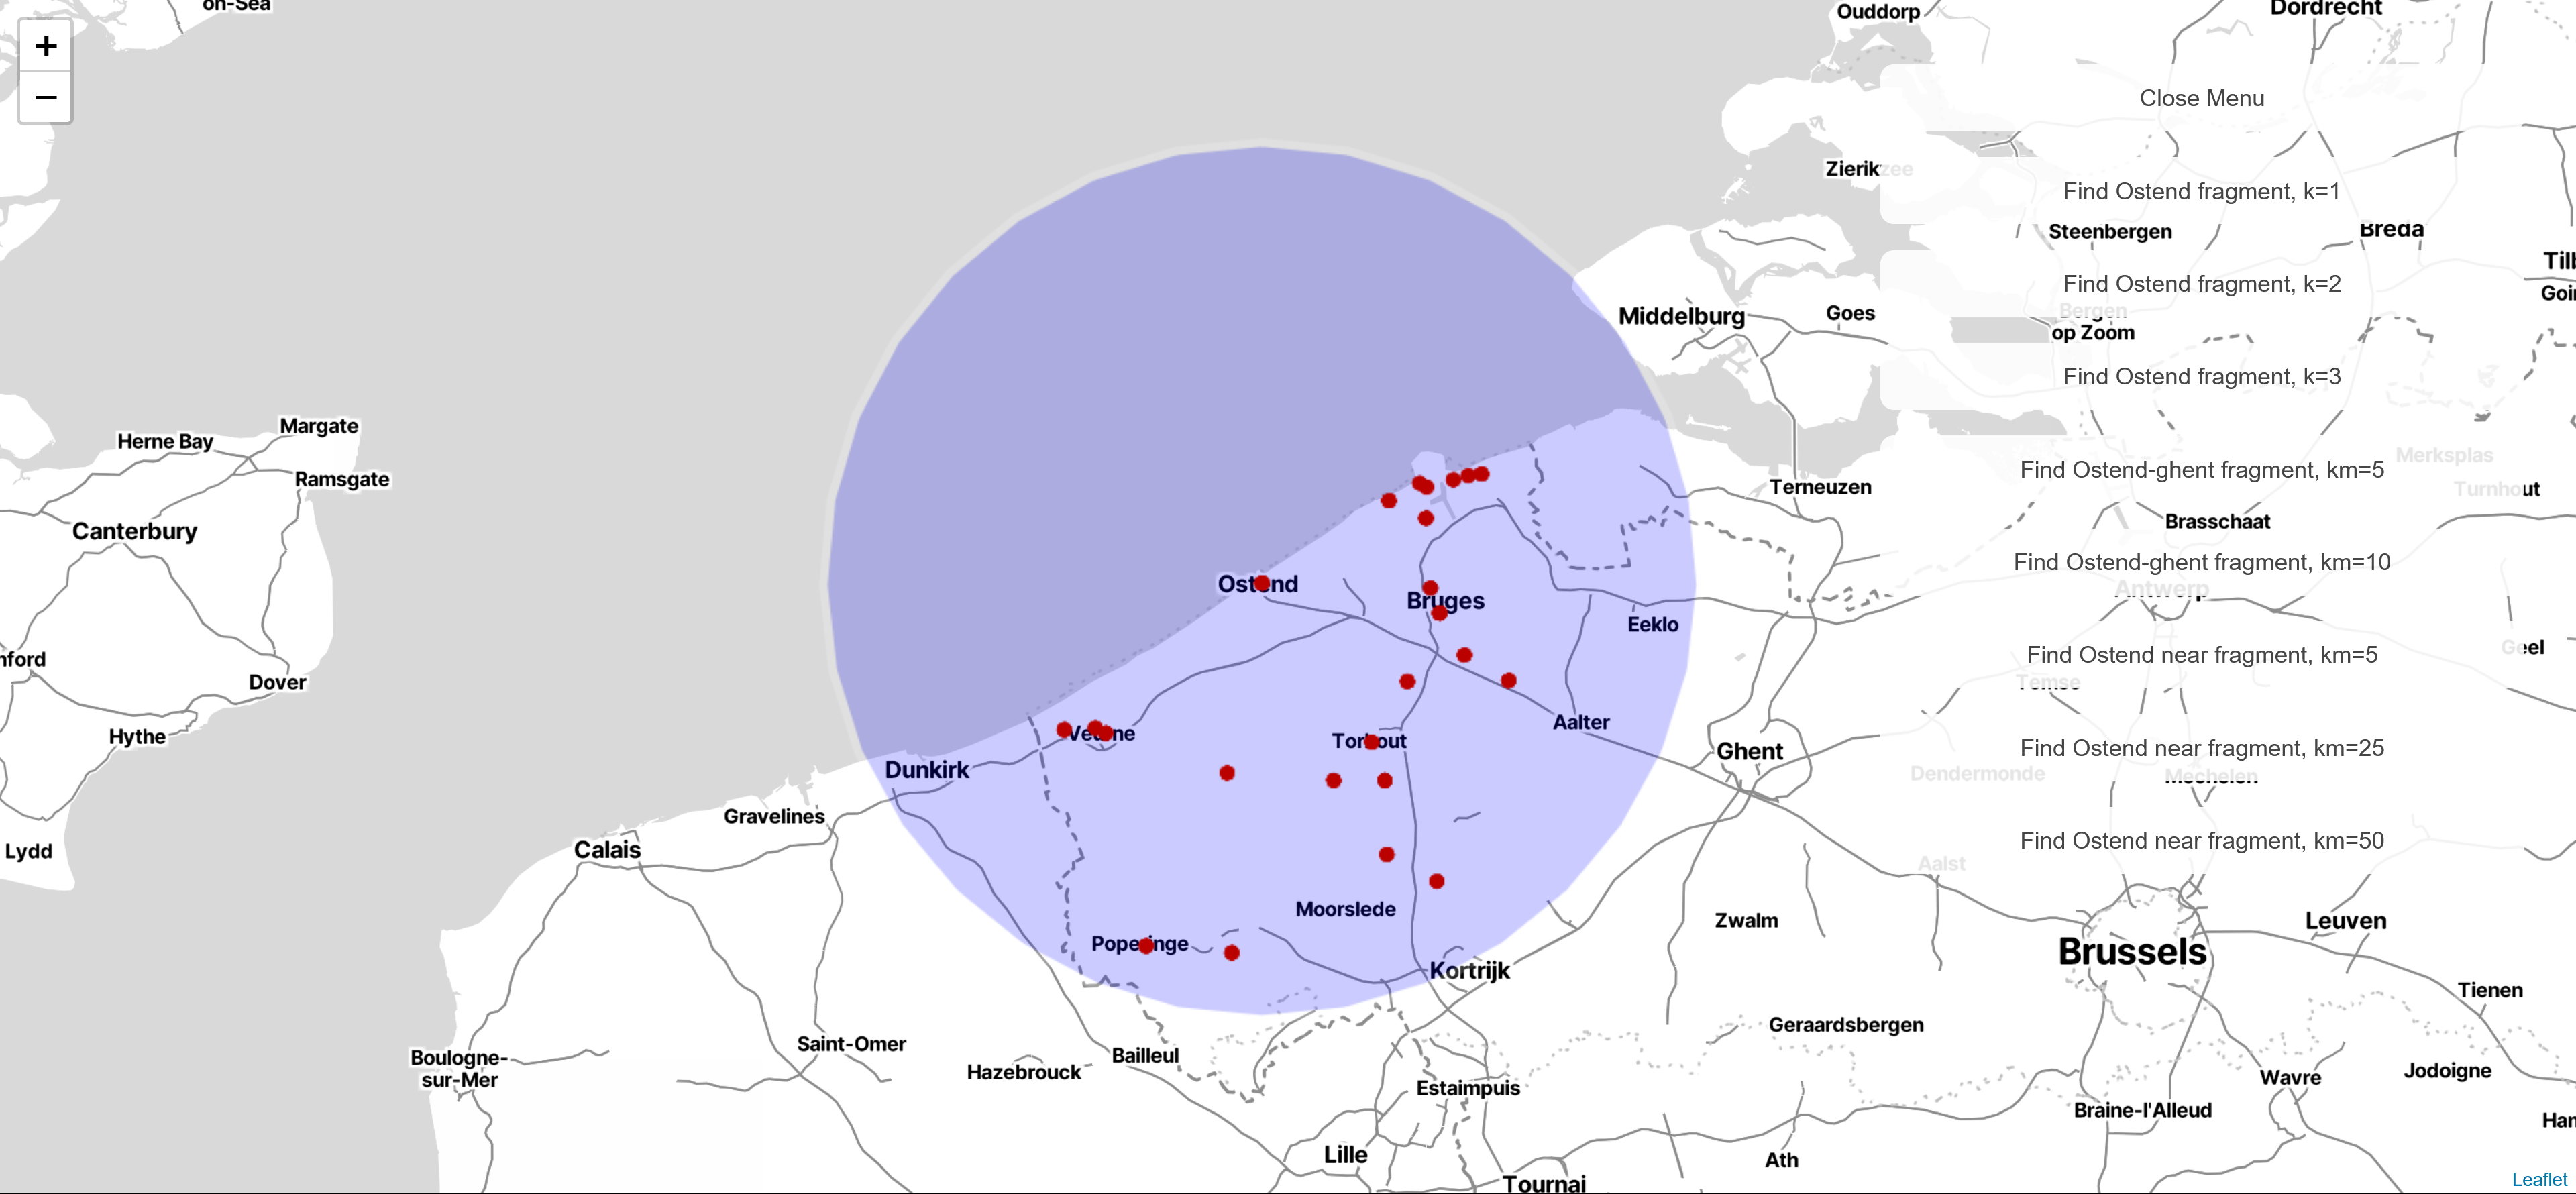
\includegraphics[width=\textwidth]{images/near visualized.png}
    \caption{Visualisation of the near fragment around Ostend with a radius of 50KM}
    \label{fig:near-visualized}
\end{figure}
\subsection{Within}
A second strategy is to work with both our source and target stations. Since we have both coordinates, we can easily create a Linestring. That is an \glsxtrshort{geojson} structure that represents a line on a map. We buffer that string to create a Polygon and select every scheduled stop point in this shape.

We use the $\$within$ \cite{noauthor_geowithin_nodate} operator of MongoDB. Like the $\$near$, we must create a special geospatial index, which requires \glsxtrshort{geojson} data.

This strategy suffers from drawbacks similar to those of near-strategy. It requires \glsxtrshort{geojson} data and a 2dsphere index. Of course, we still do not test if a scheduled stop point is reachable. So, the result could contain stop points that should not be sent to the client. 

However, compared with the near strategy. It could be that all necessary scheduled stop points are in the Polygon/fragment. This will probably depend on the hierarchy. The fragment often has many or all needed stops for long-distance train travel in a more local, e.g. city, bus network. This could quickly fall short. An example is when a bus drives in a loop, and the source and target station are far apart. This can be mitigated by choosing an appropriate buffer size or adapting one.

\begin{figure}[H]
    \centering
    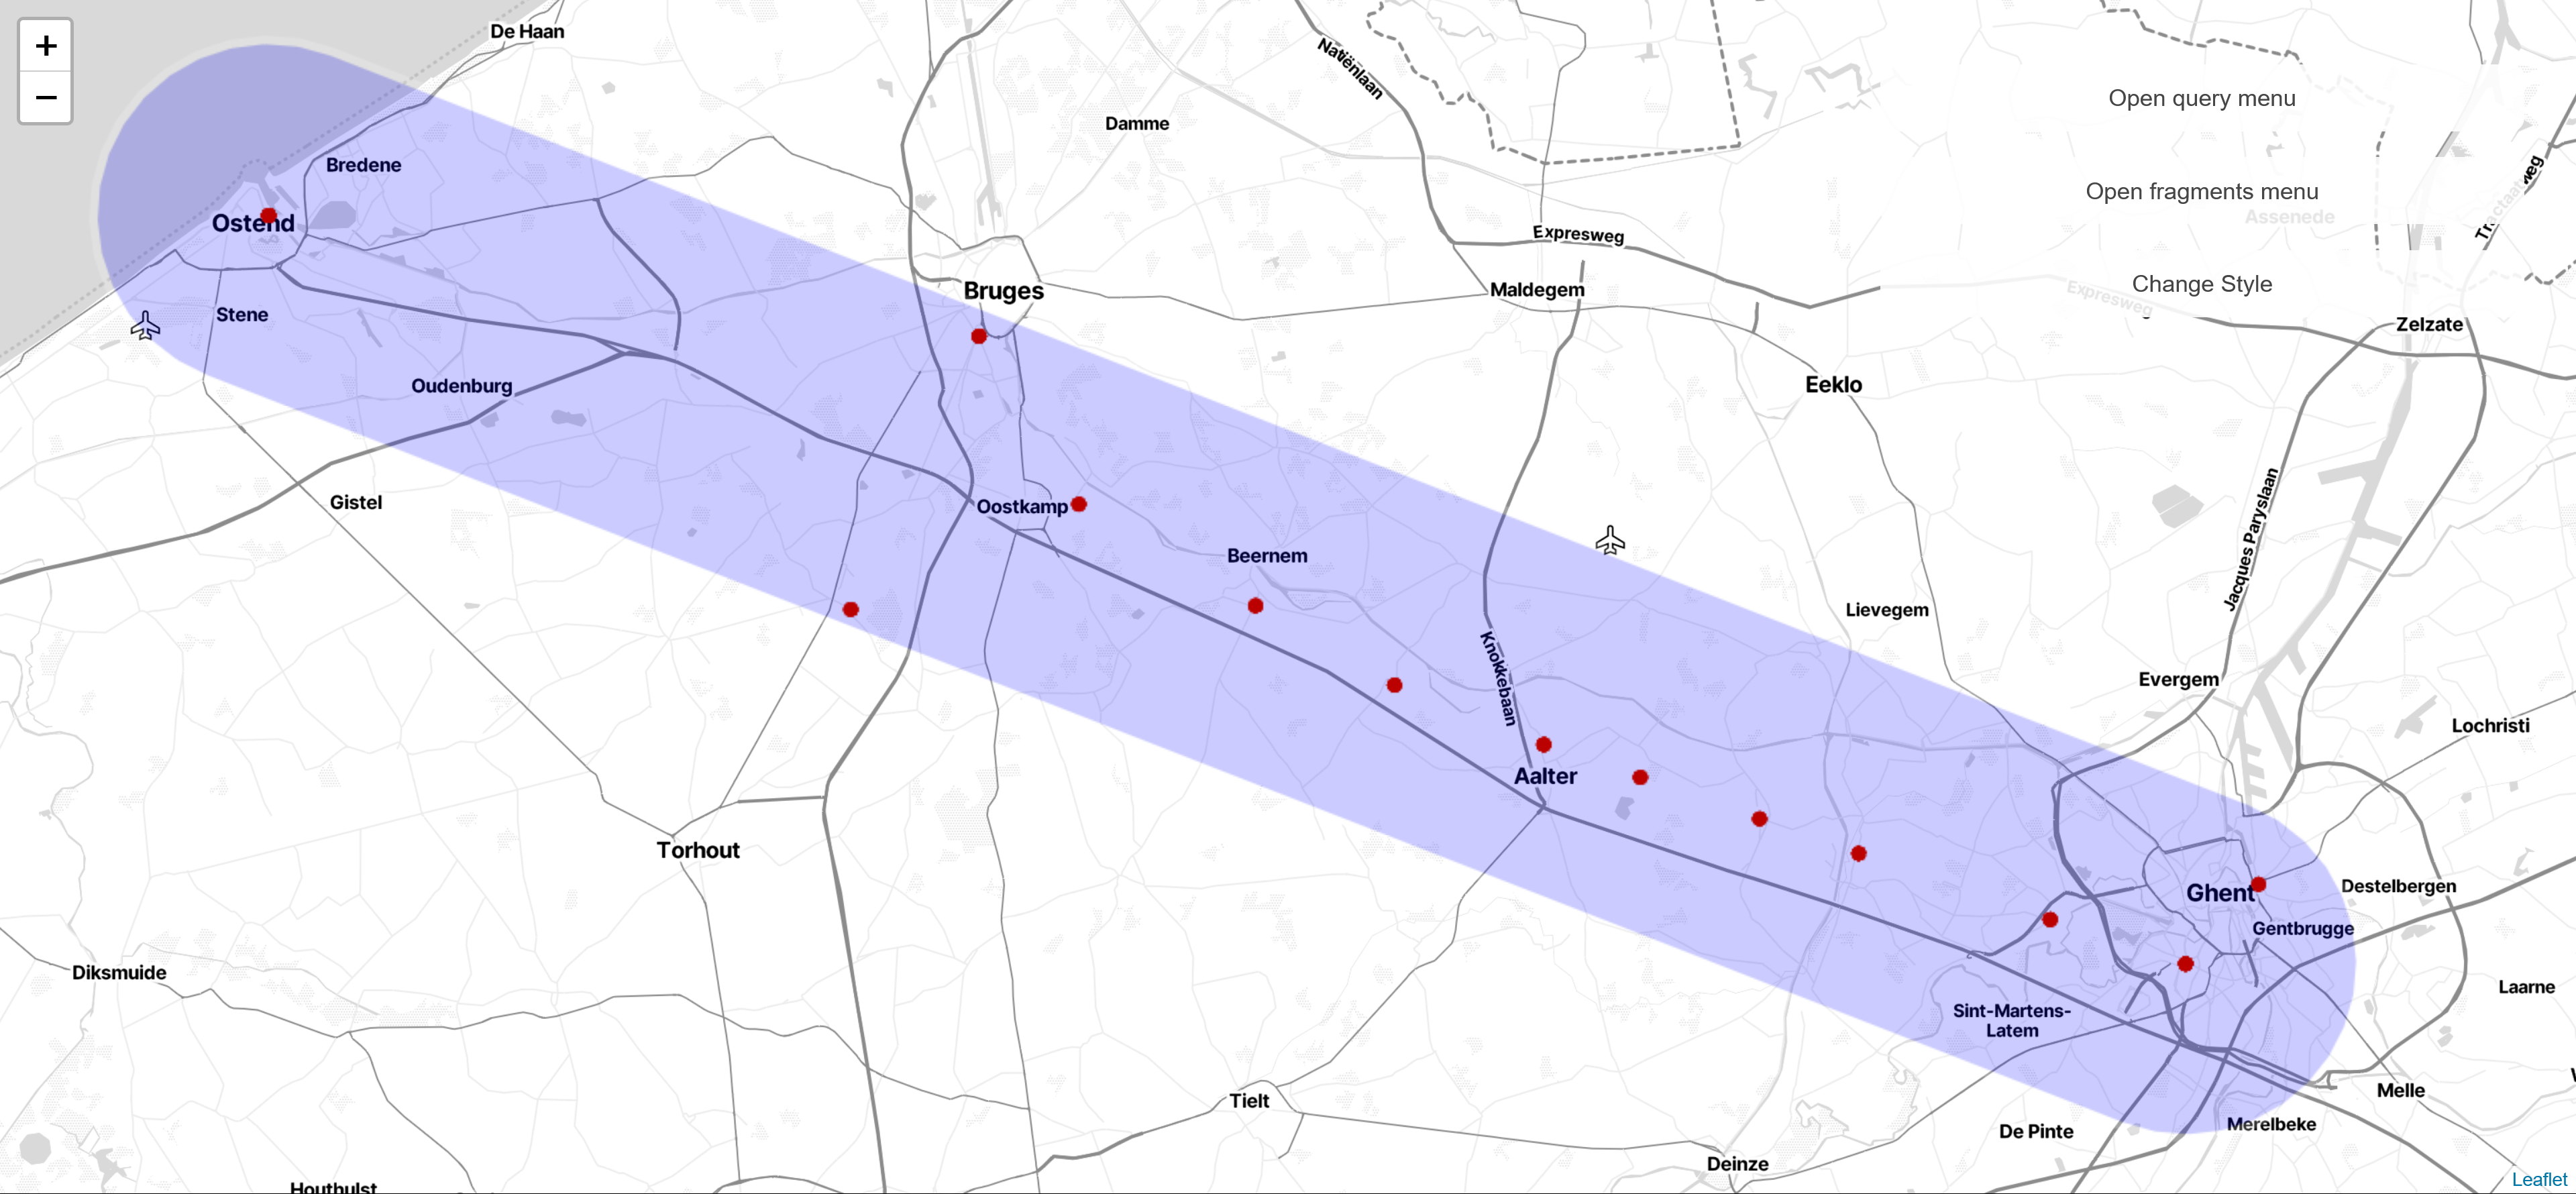
\includegraphics[width=\textwidth]{images/within visualized.png}
    \caption{Visualisation of the within fragment between Ostend and Ghent with a radius of 5KM}
    \label{fig:within-visualized}
\end{figure}

\subsubsection{Implementation}
We begin with retrieving the documents for both the source and target nodes. These coordinates in an array create a line string that we buffer. Since MongoDB does not support this kind of geo-operations, we use Turf\cite{noauthor_turfjs_nodate}.

\begin{listing}[H]
    \inputminted[linenos,frame=single,breaklines]{TypeScript}{code/turf.ts}
    \caption{Implementation of buffer lineString using the Turf library.}
\end{listing}

This buffer provides new coordinates that form a new Polygon. We can now use that polygon to test if a scheduled stop point lies in an area that is between our source and the target node.

\begin{listing}[H]
    \inputminted[linenos,frame=single,breaklines]{TypeScript}{code/within.ts}
    \caption{Implementation of the "within" fragment strategy using the $\$within$ operator.}
\end{listing}

\subsection{Reachable neighbours}
This strategy does not use MongoDB geospatial queries, so no index or geodata are needed. \\We use the $\$graphLookup$ \cite{noauthor_graphlookup_nodate} operator of MongoDB. The operator performs a recursive search. The API also allows the depth to be restricted or a branch to be stopped early when a given condition is met. 

It works by following these steps;
\begin{itemize}
    \item Takes documents as input, the start of aggregation pipeline.
    \item Targets the search to the collection designated by the from parameter.
    \item The search begins for each input document. The field's value defined by "startWith" is used for the search.
    \item It matches the field value designated by connectToField in other documents in the "from" collection.
    \item For each matched document, it adds it to an array in the original document. 
    \item This recursively continues until no document is matched or the maximum depth is reached.
    \item Return results
\end{itemize}

In this approach, it is clear we immediately test whether another scheduled stop point is reachable. We consider only trips that leave a given station and arrive at another station.

\begin{figure}[H]
    \centering
    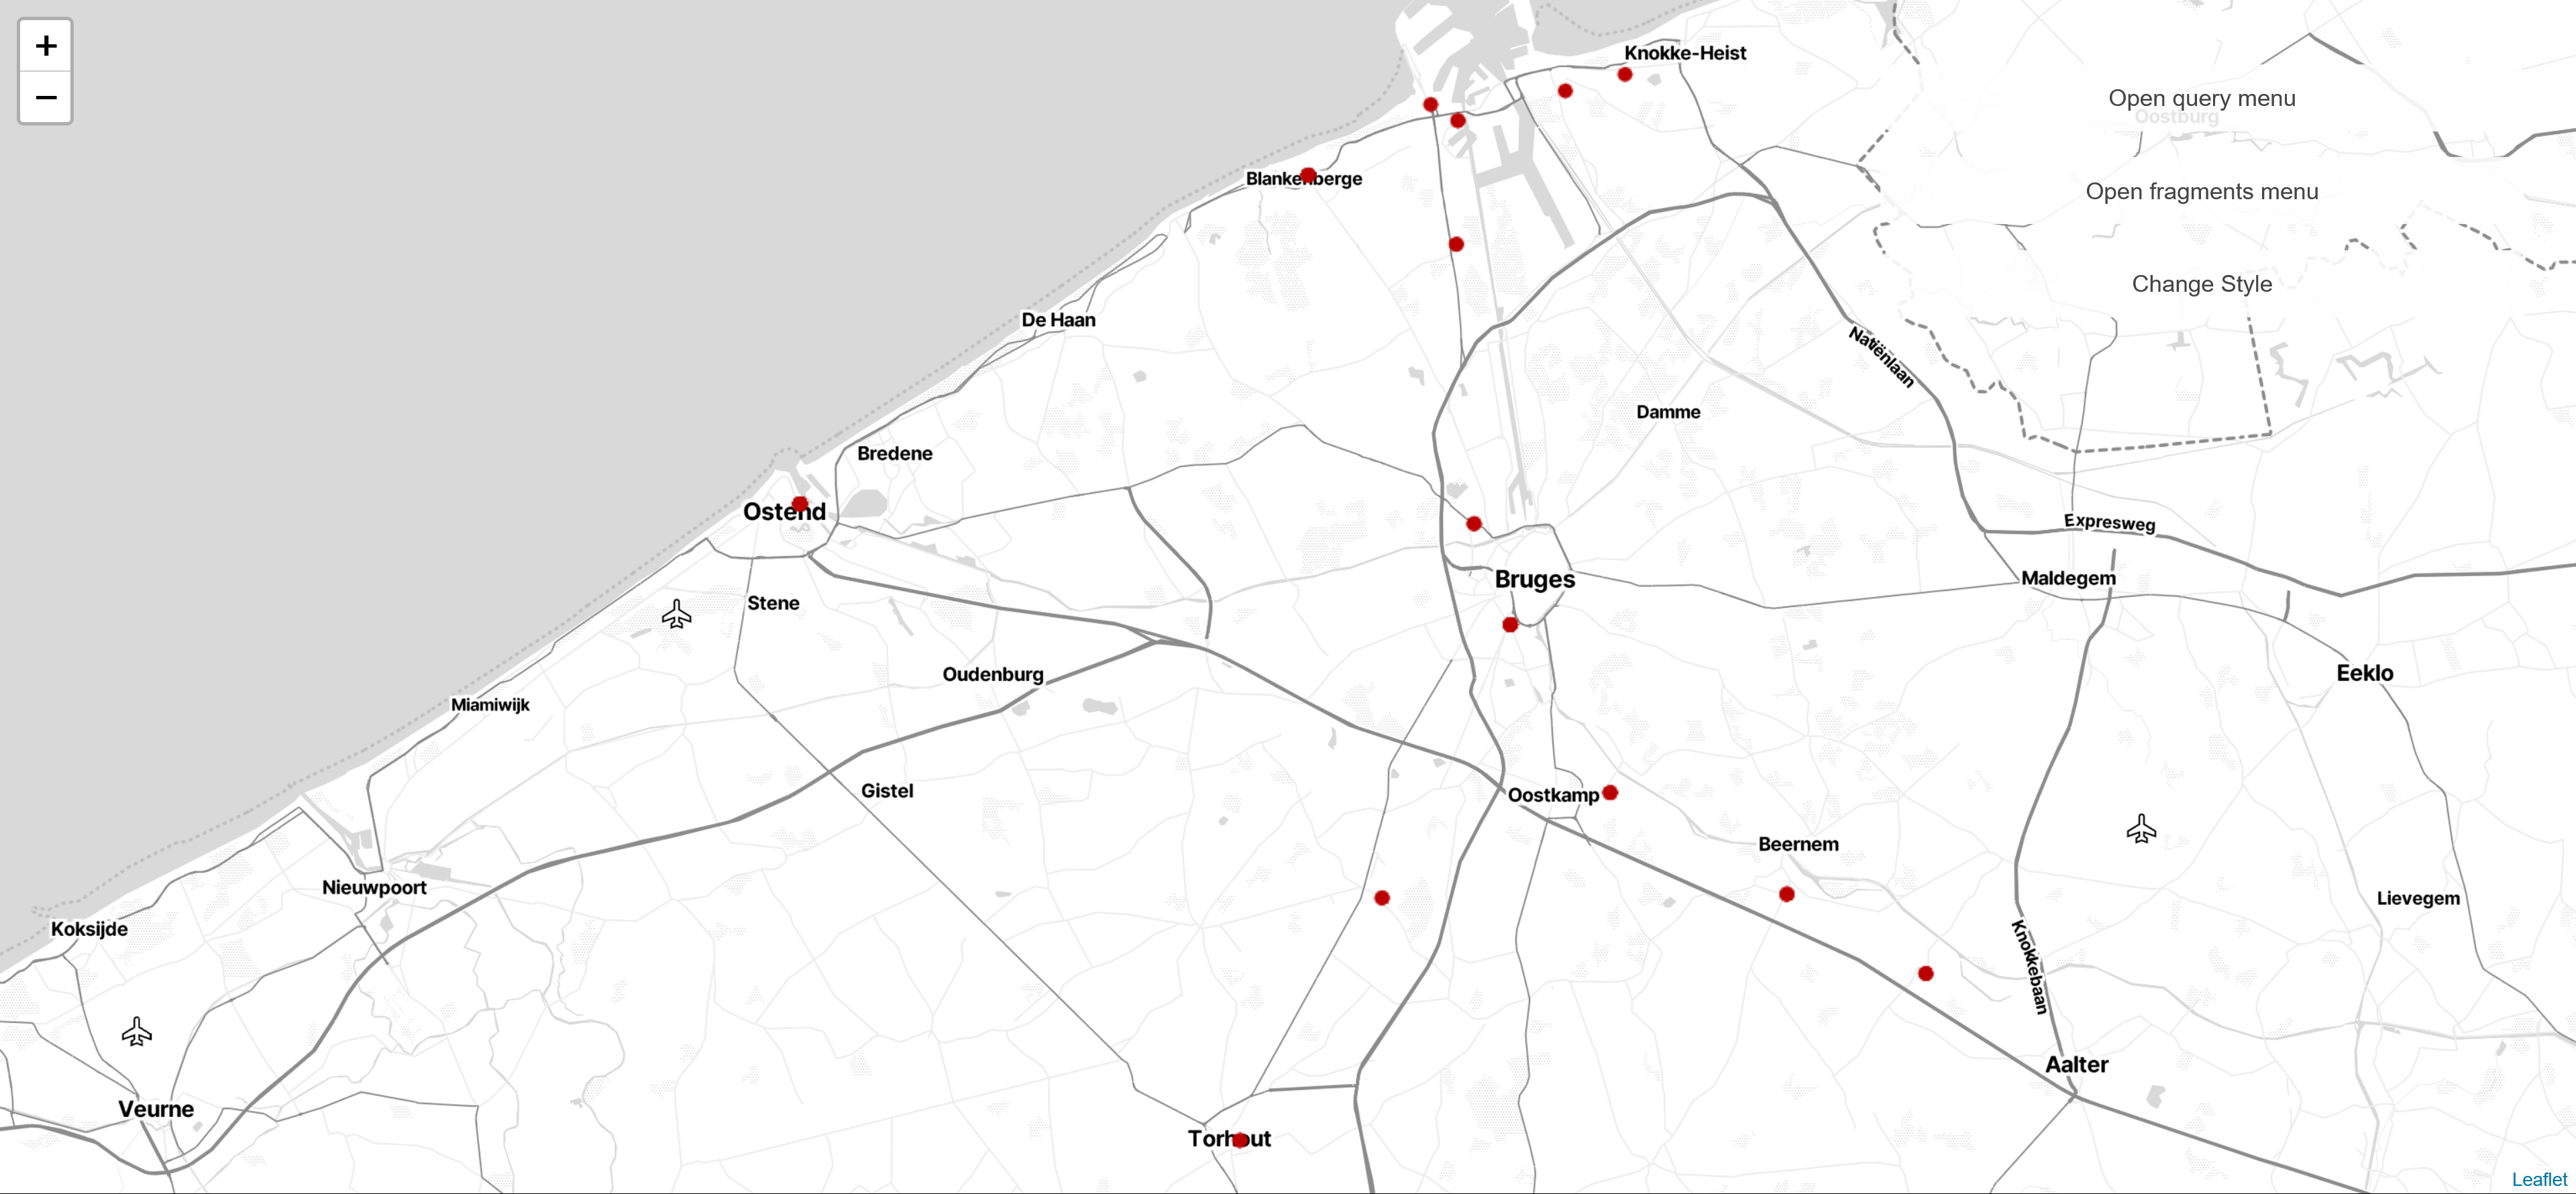
\includegraphics[width=\textwidth]{images/reacable visualized.png}
    \caption{Visualisation of the reachable fragment from Ostend with a depth of two}
    \label{fig:reachable-visualized}
\end{figure}

\subsubsection{Implementation}
Implementation is done in an aggregation pipeline, which results in a slightly more complicated pipeline. But we do not need to retrieve any document in a separate query. 

\begin{listing}[H]
    \inputminted[linenos,frame=single,breaklines]{TypeScript}{code/reachable.ts}
    \caption{Implementation of the "reachable neighbours" fragment strategy using the \\$\$graphLookup$ operator.}
\end{listing}

After that, we get one document with a field "neighbours." This array holds every connected scheduled stop point until depth k is reached. 

To convert this to one array, we run the following small code. 
\begin{listing}[H]
    \begin{minted}[linenos,frame=single,breaklines]{TypeScript}
        let list: any[] = [...t.neighbours]
        delete t["neighbours"]
        list.push(t)
    \end{minted}
    \caption{Post-processing of the $\$graphLookup$}
\end{listing}

This post-processing comes with a minor latency penalty.

\subsubsection{Implementation 2}
The first implementation has one big drawback. Mainly, MongoDB has a \glsxtrfull{BSON} limit of 16 megabytes for each document. Since graph lookup puts each neighbour in an array, this creates enormous problems. The Brussels station has many connections, so Graphlookup tries to place each document into the array. But on average, a Scheduled stop point with his passing times is around 300Kb in our dataset (\autoref{tab:mongodbstatres}). This means it quickly reaches the 16 MegaByte limit. 

We can implement the "graphlookup" pipeline using TypeScript and a for loop to avoid that. 

\begin{listing}[H]
    \inputminted[linenos,frame=single,breaklines]{TypeScript}{code/one_lookup_pipeline.ts}
    \caption{The output of this function is equal to graph lookup with depth = 0}
    \label{code:reachablejsimplementation}
\end{listing}


\subsection{Precomputed reachable neighbours}
Using the second implementation, we could precompute the reachable fragmentation strategy to speed up response times. To accomplish this, we changed \autoref{code:reachablejsimplementation}. After each loop iteration, we have a list of reachable neighbours with a k depth. We insert that list into a document. 

\begin{listing}[H]
    \begin{minted}[frame=single,linenos,breaklines]{JSON}
{
  "_id": "http://localhost:4600/1710486358000/GeplandStopPunt/8400530/k0",
  "neighbours": [
    "http://localhost:4600/1710486358000/GeplandStopPunt/8400530",
    "http://localhost:4600/1710486358000/GeplandStopPunt/8821105",
    "http://localhost:4600/1710486358000/GeplandStopPunt/8400131",
    "http://localhost:4600/1710486358000/GeplandStopPunt/8400526",
    "http://localhost:4600/1710486358000/GeplandStopPunt/8400561",
    "http://localhost:4600/1710486358000/GeplandStopPunt/8400058"
  ]
}
    \end{minted}
\end{listing}

When we want to retrieve all neighbours of a Stop point, we append the desired k-depth to the ID. We then retrieve the list and return all neighbours using find.

This last step comes with a little more complexity. We can use MongoDB's $\$in$- operator to check if the $\_id$ is in a given array of values and, if so, return the found document. However, this operator has a downside: it can not use indexes. A workaround combines the $\$or$ and $\$eq$ operators.
\begin{listing}[H]
\begin{minted}[linenos,breaklines,frame=single]{TypeScript}
return collection.find({
        $or: neighbours.map((el) => {
            return {_id: {$eq: el}}
        })
    }, {projection: {gepjson: 0}}).toArray();
\end{minted}
\caption{Retrieval of the precomputed neighbours.}
\end{listing}
\subsection{Combination of precomputed reachable neighbours and within.}
Here, we combine two fragmentation strategies. Code-wise, this is not hugely different from the previous implementations. But should allow for within to operator be faster, since the operator now works on a limited set of stations. The goal is to have only reachable stations but also focus more on relevancy. 
\begin{figure}[H]
    \centering
    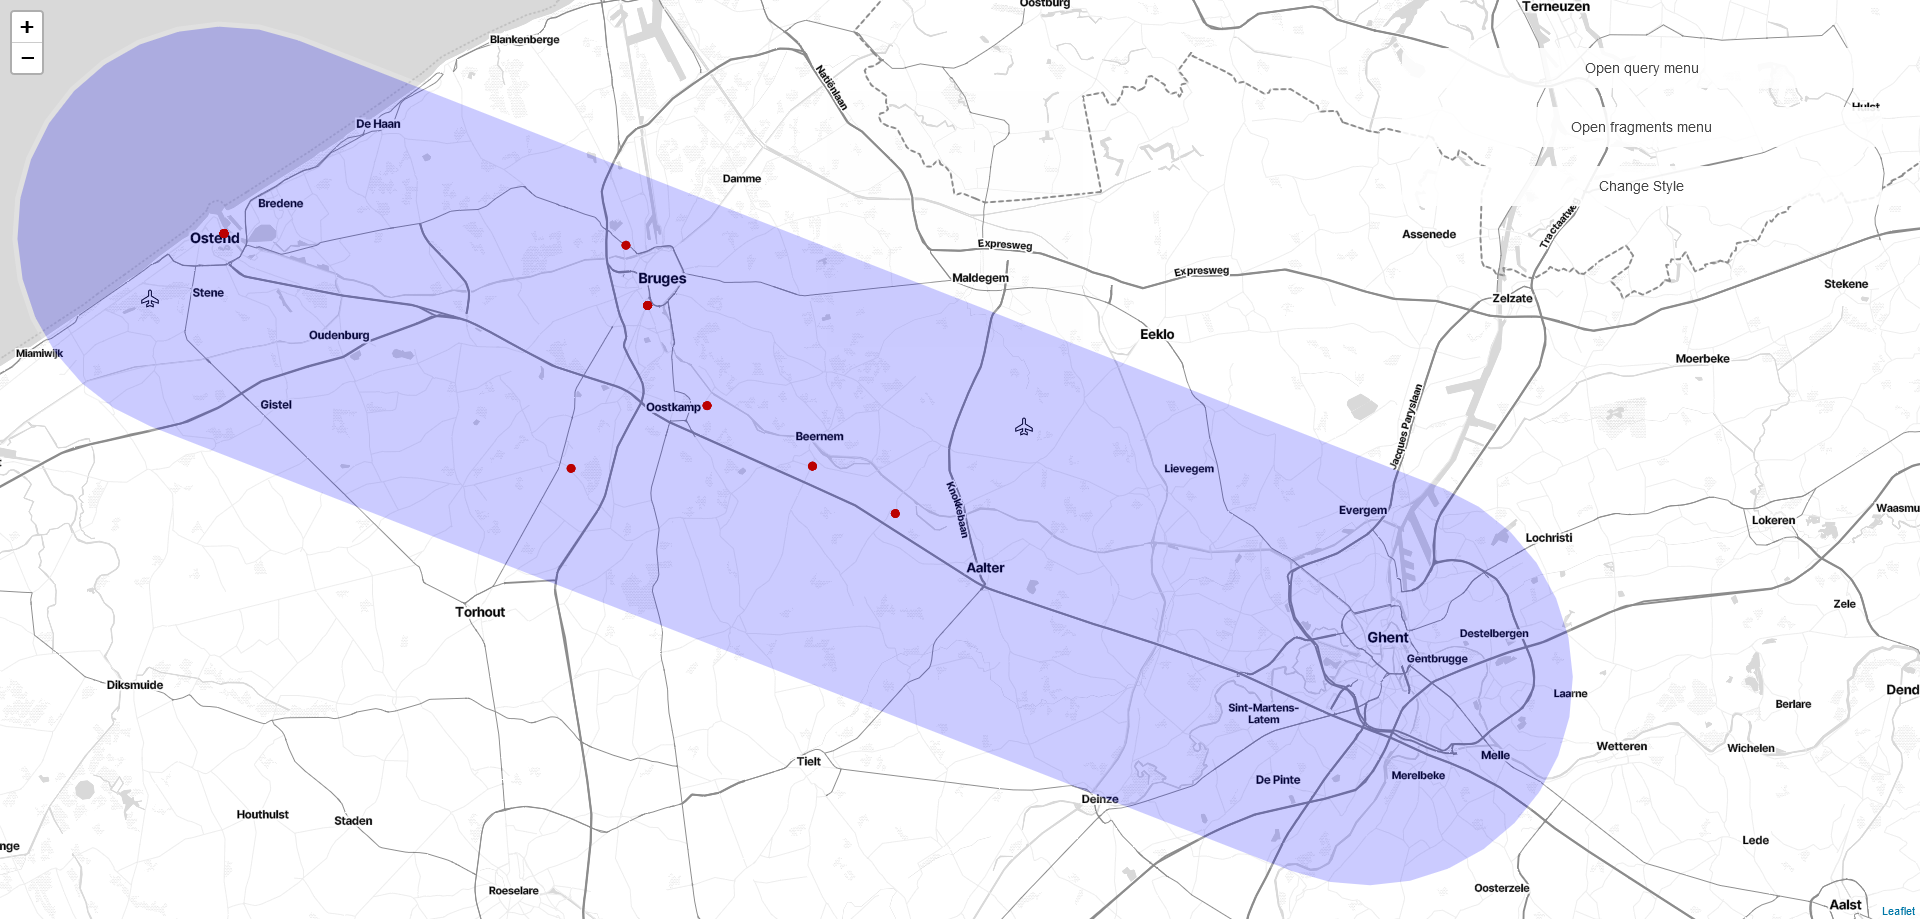
\includegraphics[width=\textwidth]{images/precomputed within.png}
    \caption{At first sight, this is not so different from within, but fewer stations are included.}
    \label{fig:precomputedwithin}
\end{figure}
\subsection{Overview}
\begin{table}[H]
\centering
\begin{tabular}{|l|l|l|l|l|l|}
\hline
\textbf{} &
  \textbf{near} &
  \textbf{withIn} &
  \textbf{\begin{tabular}[c]{@{}l@{}}reachable \\ neighbours\end{tabular}} &
  \textbf{\begin{tabular}[c]{@{}l@{}}precomputed \\ reachable neighbours\end{tabular}} &
  \textbf{\begin{tabular}[c]{@{}l@{}}precomputed \\ reachable neighbours \\and whitin\end{tabular}} \\ \hline
\textbf{GeoJSON required} & \cellcolor[HTML]{FD6864}yes & \cellcolor[HTML]{FD6864}yes & \cellcolor[HTML]{67FD9A}no  & \cellcolor[HTML]{67FD9A}no & \cellcolor[HTML]{67FD9A}no \\ \hline
\textbf{New index needed} & \cellcolor[HTML]{FD6864}yes & \cellcolor[HTML]{FD6864}yes & \cellcolor[HTML]{67FD9A}no  & \cellcolor[HTML]{67FD9A}no & \cellcolor[HTML]{67FD9A}no  \\ \hline
\textbf{\begin{tabular}[c]{@{}l@{}}Fragment can contain\\ unreachable stations\end{tabular}} &
  \cellcolor[HTML]{FD6864}yes &
  \cellcolor[HTML]{FD6864}yes &
  \cellcolor[HTML]{67FD9A}no &
  \cellcolor[HTML]{67FD9A}no &
  \cellcolor[HTML]{67FD9A}no \\ \hline
\textbf{independant of MongoDB api}      & \cellcolor[HTML]{FD6864}no & \cellcolor[HTML]{FD6864}no & \cellcolor[HTML]{FD6864}no  & \cellcolor[HTML]{67FD9A}yes& \cellcolor[HTML]{FD6864}no \\ \hline
\textbf{Can be calculated at runtime}          & \cellcolor[HTML]{67FD9A}yes & \cellcolor[HTML]{67FD9A}yes & \cellcolor[HTML]{67FD9A}yes & \cellcolor[HTML]{FD6864}no & \cellcolor[HTML]{FD6864}no  \\ \hline
\end{tabular}
\caption{Overview of fragment strategies.}
\label{tab:strategies}
\end{table}
To sum up our fragmentation story, we see that no real low-latency solution allows runtime computation. Furthermore, the first two strategies are largely dependent on MongoDB API. Although a similar functionality for other database systems exists \cite{noauthor_postgis_nodate}, it is more difficult to replicate. The reachable neighbours are implemented using \glsxtrshort{js} and basic MongoDB \glsxtrshort{api} (find). 

The geospatial strategies do not account for reachability; hence, they can contain stations not reachable by our origin node or any node connected to our origin. This can waste network bandwidth. However, the reachable neighbour's strategy can contain irrelevant stations. For example, when connected stations are included, they are entirely in the wrong direction of our destination node. 

\subsubsection{Compression}
It immediately became apparent that there are many Scheduled Stop Points caused by the fact that stations have multiple platforms. This quickly adds to many bytes, as seen in \autoref{fig:fragsize}, even if we chose a low depth for the reachable neighbour's strategy.

One way to mitigate this is to enable compression express middleware\cite{noauthor_compression_2019}. Using the default options, the response will be compressed before sending if the threshold of 1Kb has been reached. When the client receives the data, it will uncompressed. 

Compression and decompression have adverse effects on response time. However, large transfers are significantly reduced in size and time. 

\section{Demo}\label{sec:demo}
Since the \glsxtrshort{raptor} has been browserified to run in the browser, it is pretty quick to develop a demo web app.

For this, we use some libraries and services:
\begin{itemize}
    \item \textbf{Leaflet} \cite{noauthor_leaflet_nodate}: It is an open-source library to create mobile-friendly interactive maps. It's lightweight, flexible, and easy to use. Leaflet supports a variety of mapping providers, including OpenStreetMap and Mapbox, and offers powerful features for adding markers, popups, and layers to your maps. It is used to overlay our results onto an OpenStreetMap map. 
    \item \textbf{GeoJSON-vt} \cite{noauthor_mapboxgeojson-vt_2024}: This library specialises in creating vector tiles from GeoJSON data. It's designed to handle large geographic data sets efficiently and facilitate displaying detailed maps in web applications. 
    \item \textbf{Leaflet-Geojson-vt} \cite{kshetri_iamteksonleaflet-geojson-vt_2024}: A plugin for Leaflet to use GeoJSON-vt.
    \item \textbf{Turf.js} \cite{noauthor_turfjs_nodate}: Turf.js is a JavaScript library providing geospatial functions for geographic data. It includes features for performing various geospatial operations, such as calculating distances and manipulating GeoJSON objects. They are used to add visualisations for the fragments strategies.
\end{itemize}

An online demo has been placed on \url{https://mx2.tibovanheule.space/raptor/}\footnote{This is not my fastest server, please be patient.}.

\chapter{Evaluation}
\chaptermark{Evaluation}
\addcontentsline{toc}{chapter}{Evaluation}  

Preprocessing time, space consumption of the precomputed auxiliary data, query processing time and space, the ability for multi-criteria optimization (travel times, number of transfers, prices, etc.), realistic modelling (transfer buffers, footpaths), and the ability to deal with delays and other real-time information.
\section{MongoDB Storage}
We created a merged view for our entry point. The connected entities are embedded in our scheduled stop point. This ensures we can quickly look up each station using \glsxtrshort{raptor}.

However, we also added the rest of the information to separate collections of MongoDB. This ensures we can look up information after route planning. You can get either the entity alone or an entity and all its referenced entities. They are returned as a graph and are not embedded. The code for resolving all the references in an entity can be found in \autoref{code:resolve}. An example can be found in \autoref{code:example:line}.

\begin{table}[H]
\centering
\begin{tabular}{|l|l|l|l|l|l|}
\hline
\textbf{} &
  \textbf{\begin{tabular}[c]{@{}l@{}}Number of\\  documents\end{tabular}} &
  \textbf{\begin{tabular}[c]{@{}l@{}}Avg. \\ document size\end{tabular}} &
  \textbf{\begin{tabular}[c]{@{}l@{}}Number \\ of indexes\end{tabular}} &
  \textbf{\begin{tabular}[c]{@{}l@{}}Total\\  index size\end{tabular}} &
  \textbf{\begin{tabular}[c]{@{}l@{}}Total\\ storage size\end{tabular}} \\ \hline
AutoriteitOfOperator   & 1    & 134B     & 1 & 20.48kB  & 20.48kB  \\ \hline
Dienstkalender         & 9.7K & 24.71kB  & 1 & 151kB    & 151.57MB \\ \hline
Dienstrit              & 37K  & 309B     & 1 & 831.49kB & 2.05MB   \\ \hline
Dienstritpatroon       & 37K  & 2.27kB   & 1 & 811.01kB & 10.83MB  \\ \hline
Doorkomsttijd          & 652K & 216B     & 1 & 9.22MB   & 15.26MB  \\ \hline
Lijn                   & 856  & 479B     & 1 & 28.67kB  & 73.73kB  \\ \hline
Merged                 & 2.6K & 301.22kB & 5 & 31.07MB  & 67.70MB  \\ \hline
Route                  & 856  & 4.82kB   & 1 & 28.67kB  & 733.18kB \\ \hline
Stopplaats             & 2.6K & 209B     & 1 & 7373kB   & 98.30kB  \\ \hline
StopplaatsInRitpatroon & 652K & 715B     & 2 & 17.79MB  & 45.39MB  \\ \hline
\end{tabular}
\caption{Statistics in MongoDB of our result.}
\label{tab:mongodbstatres}
\end{table}
We can see that indexing is using a lot of storage. The problem is indexes on embedded documents, which are necessary to speed up our creation time.
% todo add implementation in appendix
\subsection{comformity of ontology}
\subsubsection{comformity application profiles}
\glsxtrshort{oslo} has also described when a \glsxtrshort{jsonld} document conforms to an application profile \cite{noauthor_conformiteit_nodate}.

An application profile is a specification for data exchange that introduces additional constraints for applying vocabularia. These constraints could include refinement of terminology (classes and properties) consistent with the semantics from the relevant specifications with a well-defined usage as a goal;
    External terminology (classes and properties) is used for new/extra terms not found in the existing vocabulary.

To conform with the \glsxtrshort{oslo} application profile, the following constraints have to be met:
\begin{itemize}
    \item \textbf{Must} each class contains the attributes that have a cardinality of one/
    \item \textbf{Forbidden} for a class attribute with a cardinality of maximum one to have more instantiations.
    \item \textbf{Forbidden} to use terminology of vocabularia not defined in the application profile.
    \item \textbf{Allowed} to use terminology in a way that is consistent with her semantics (definition, use, domain and range)
    \item \textbf{Allowed} to extend with other vocabularies that do \textbf{do not overlap} with terminology from this vocabulary. 
\end{itemize}
\subsubsection{\glsfmtfull{shacl}}

The \glsxtrshort{oslo} organisation also provides a shacl file that describes the ontology constraints. This also includes cardinality.

We tested our merged Scheduled Stop Points. First, we took one scheduled Stop point and added our context file. Then proceeded to transform the \glsxtrshort{jsonld} document to N-Quads using @rdfjs/parser-jsonld \cite{noauthor_rdfjs-baseparser-jsonld_2024}. We then read the Shacl File and provide both turtle files to the \glsxtrshort{shacl} validator \cite{noauthor_rdf-validate-shacl_2024}.

We got good results back, THe main constraint was a ClassConstraint violation. Mainly, this was caused by the fact that the entity that a \glsxtrshort{iri} was pointing to was not in the graph.

\section{Fragmentation evaluation}
We wrote a quick Python script for a first but straightforward evaluation of our fragment strategies. The duration (\autoref{fig:fragduration}) is the total duration to make a request, receive the request and do some processing from the client's viewpoint. The size (\autoref{fig:fragsize}) is the total size of a request, including headers.

For these measurements, a list of 100 stations was randomly selected out of all possible stations. For this, we used $random.choice()$. When a destination station was needed, we selected another 100 stations. Then, we made our requests to the server.

\begin{figure}[H]
    \centering
    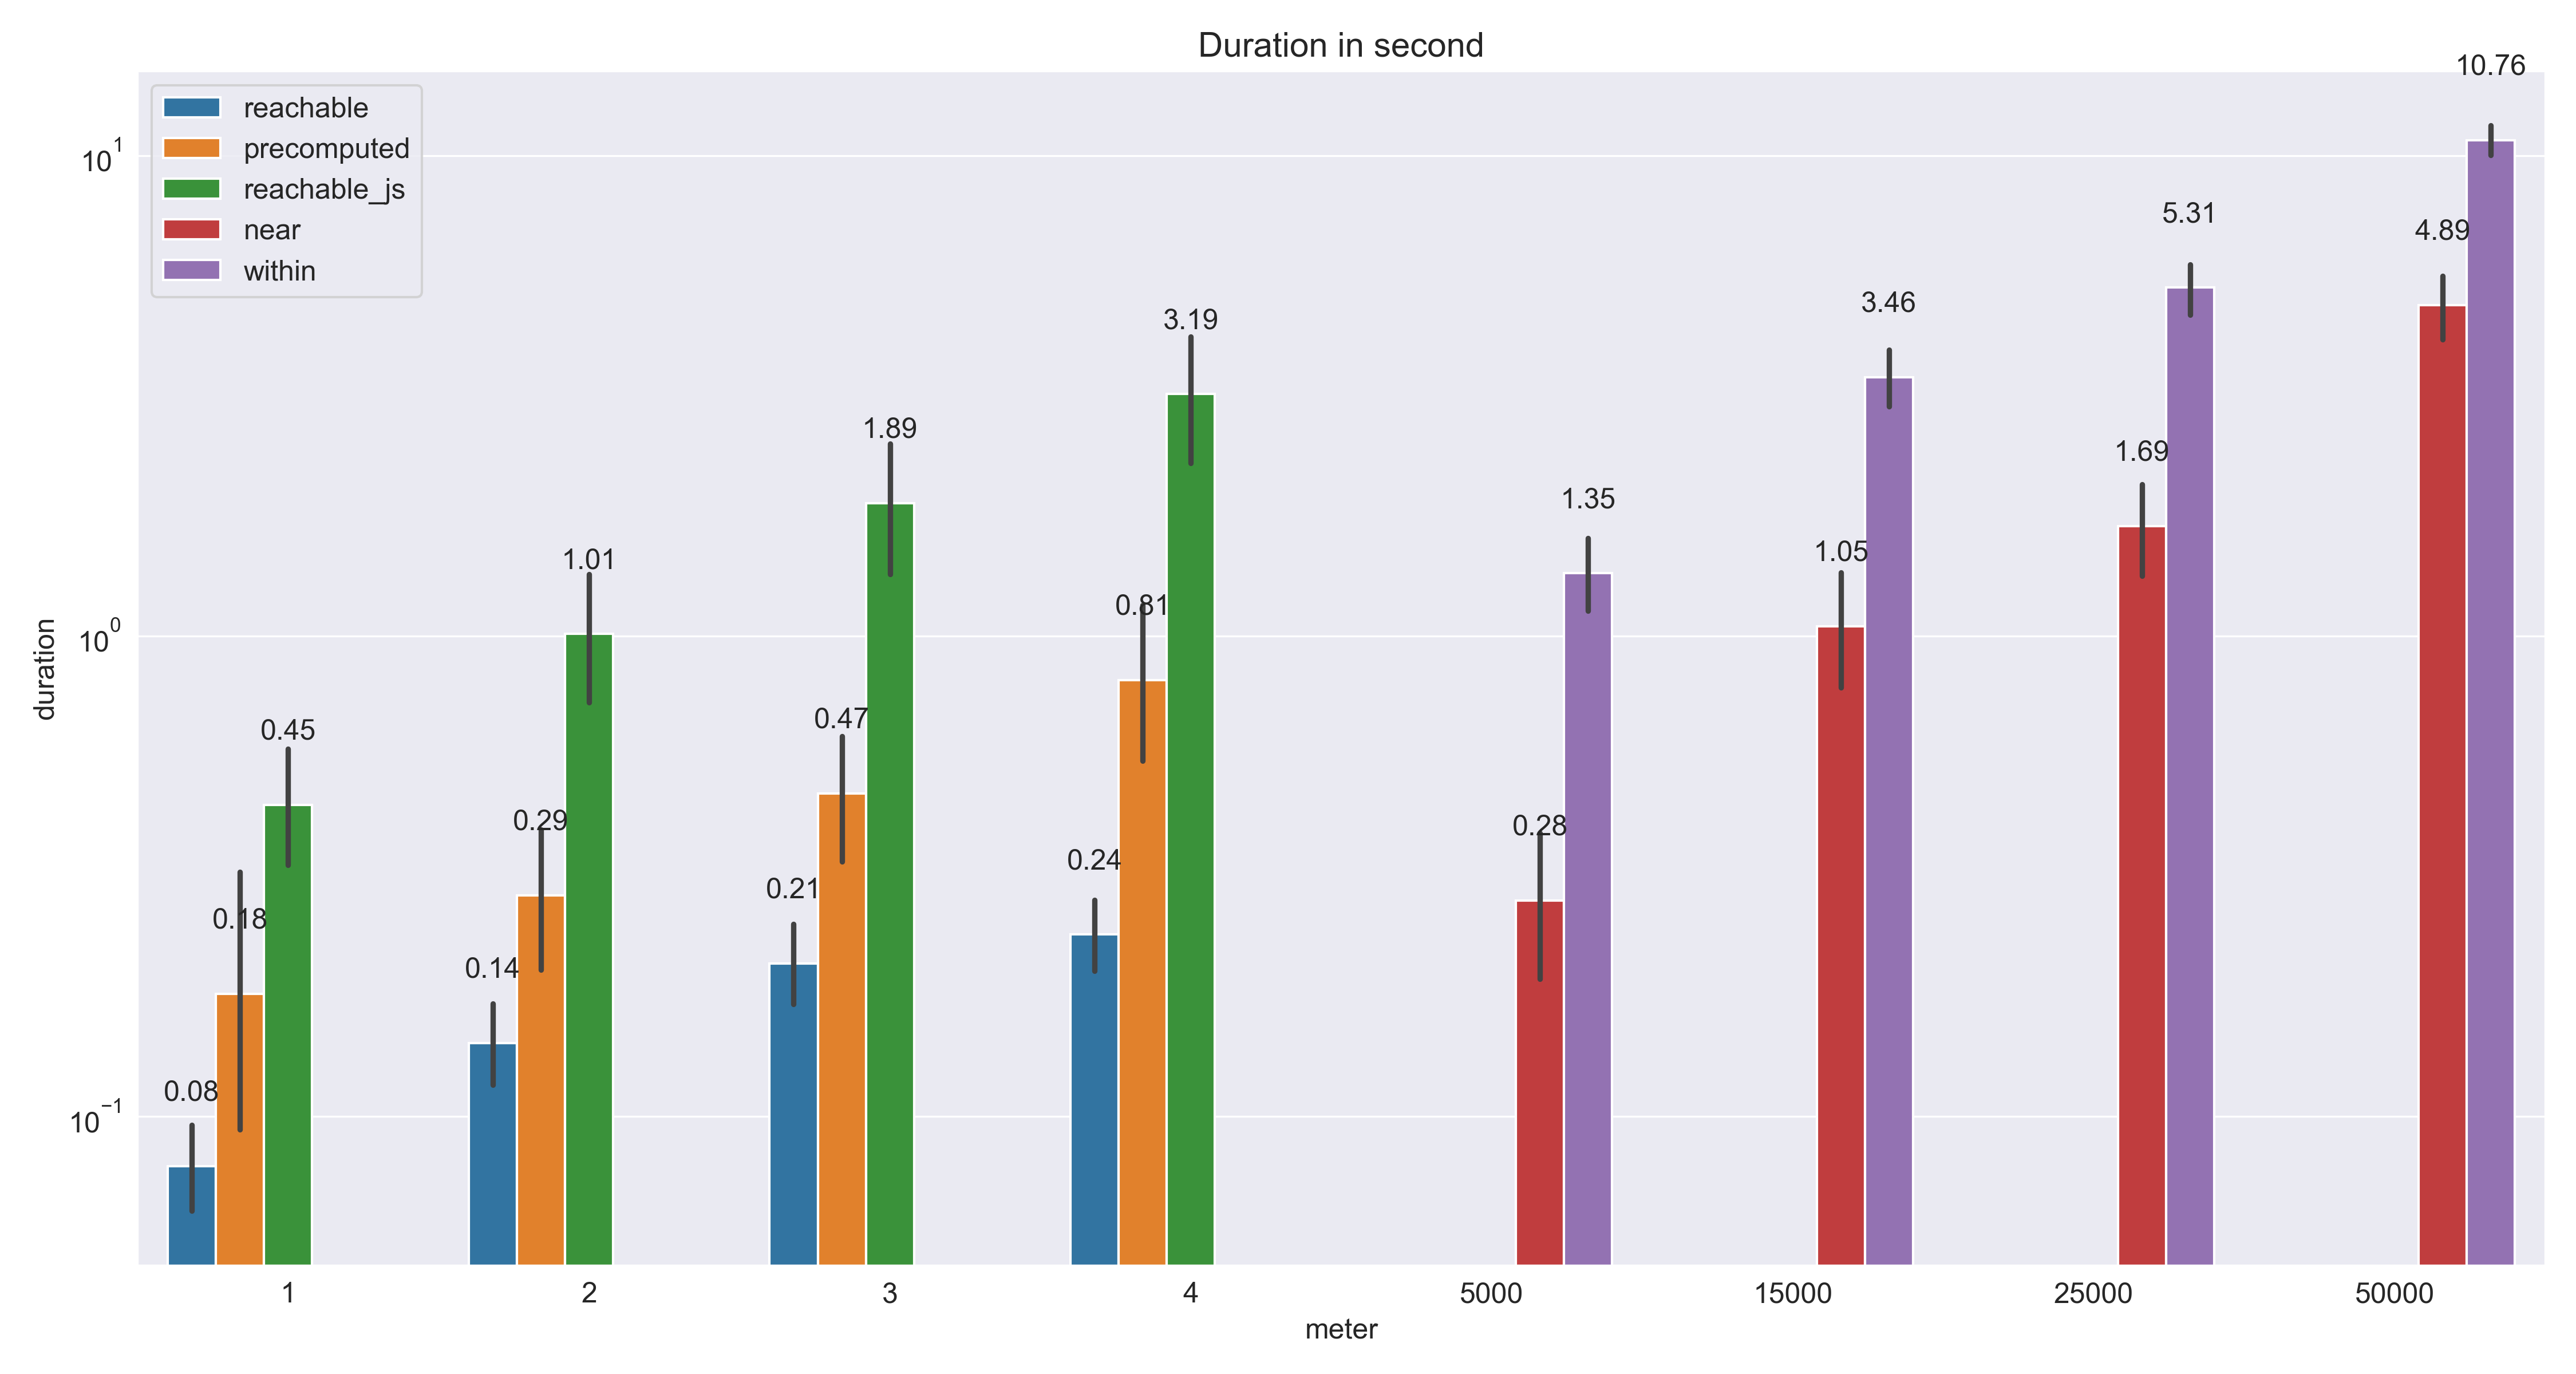
\includegraphics[width=\textwidth]{images/fragmentsbyduration.png}
    \caption{Some tests measure the response time and processing time needed to receive a fragment. The left four on the x-axis use a k as a parameter, and the right four use meters as a parameter. The Y-axis is in the log scale!}
    \label{fig:fragduration}
\end{figure}
\begin{figure}[H]
    \centering
    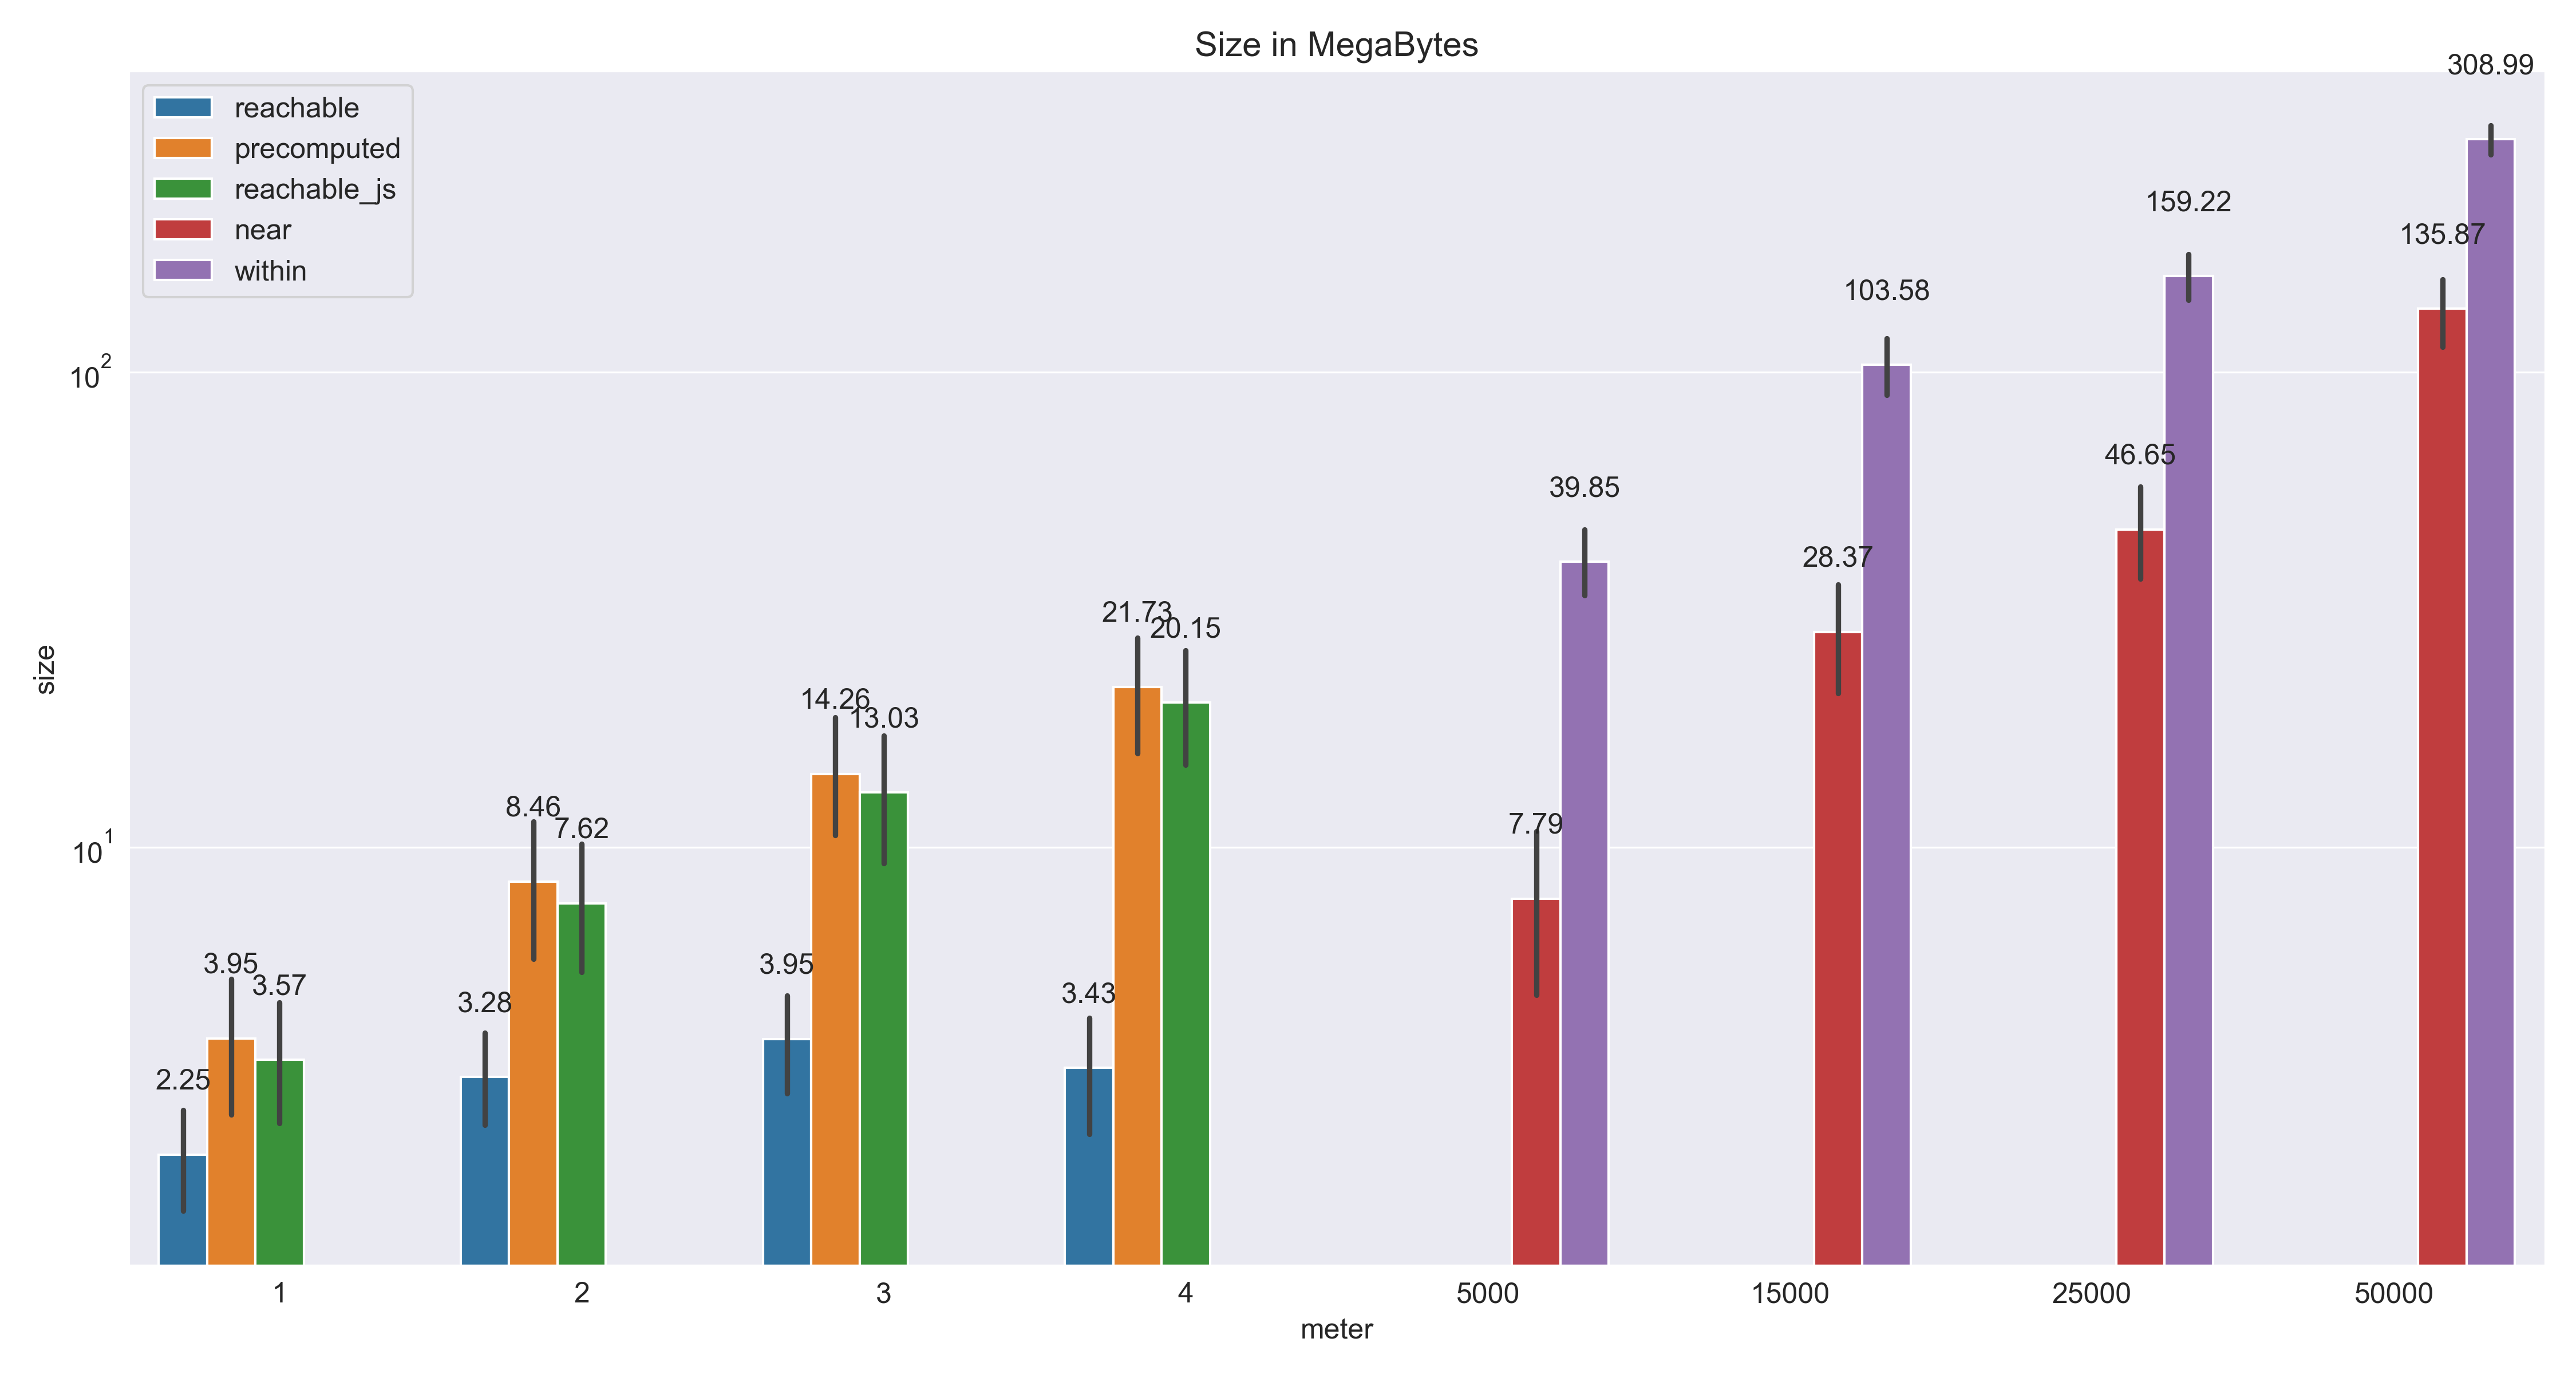
\includegraphics[width=\textwidth]{images/fragmentsbysize.png}
    \caption{Some tests to measure the size of a fragment. The left four on the x-axis use a k as a parameter, and the right four use meters as a parameter. The Y-axis is in the log scale!}
    \label{fig:fragsize}
\end{figure}


If we look at \autoref{fig:fragduration}, we see that the reachable strategy is the fastest. The JavaScript version quickly becomes slower with higher k values. The precomputed version indeed saves time compared to the javascript version. 

The reachable implementation using $\$graphLookup$ is the fastest, but we can not trust the graph as K grows. As graphlookup errors, when passing the 16 Megabyte limit, it can only handle the subset of selected stations without many connections. 

The near strategy is pretty fast, but it has trouble finding any relevant stations for small values. We must use a significant parameter for long-distance travel, selecting even more irrelevant stations. 

The within strategy is generally relatively slow and has the most size. This is logical since it typically spans a large area and, depending on the buffer size contains many stations. This is probably the leading cause of its slowness. This can be seen as an advantage and a weakness. It presumably includes a lot of relevant stations; since the chance is very high, we have to pass by a station between our source and destination stations. But presumably, it also contains a lot of stations we do not pass by. We still have fewer irrelevant stations than using the near strategy. 
\chapter*{Conclusion}
\chaptermark{Conclusion}
\addcontentsline{toc}{chapter}{Conclusion}


We see that the execution time of a query is related to the number of fragments that need to be requested and the size of those fragments.

If we compare the fragmentation evaluation \autoref{fig:fragduration}, we see correlations with the results in \autoref{fig:timestackedcuratedpersonal}, \autoref{fig:curatednmbs} and \autoref{fig:random:timstacked}. For example, let's compare the worst performer in our raptor evaluation "within". We see that this is also the worst performer in our fragmentation evaluation\footnote{Reachable\_js was not tested in our raptor evaluation}.

But as we observe \autoref{fig:timestackedcuratedpersonal}, \autoref{fig:curatednmbs} and \autoref{fig:random:timstacked} with higher $K$, strategies with too small fragments like Near with 5 km, quickly perform worse. This is due to the smaller size, which causes the Raptor algorithm to request more fragments. The overhead of more requests causes worsened performance. We can see the steep incline of requests and overlap in \autoref{fig:spentfetching}, \autoref{fig:personalrequests} and \autoref{fig:nmbsrequests}.

Choosing a perfect fragmentation strategy is complex, depending on response time, size, and overlap. For $k=1$, you should choose something small, like a buffer of 5 km or a depth of one for reachable neighbours. For higher $K$ values, the precomputed reachable combined with within is a good choice as it enables more extensive fragments than the 5 km buffer. Still, thanks to the Within, the final output size is also limited. This leaves a more in-between solution. 

Finally, we would like to mention that different strategies could be interesting with a different transportation network, such as an urban bus network. Here, we deal with a density different from that of long-distance travel. So, even though we accomplished our goals from the introduction, some experimentation and future work are still left.

\subsection*{Future work}

To further improve the response size, let the client store a list of IDs that have been seen. Using such a list for each fragmentation request could be interesting so the server can filter out stations. This would essentially remove all overlap in each fragment and further decrease the size. 

Further combinations of fragmentation could be analysed—for example, use Within only for the initial request. When a trip leads to a fragment outside the fragment, we could use one of the reachable strategies. This would also decrease a lot of overlap.

The server load, especially memory, is relatively high; a suspicion is the MongoDB driver of Node.js. Although it makes sense to write the client in \glsxtrshort{js}, it makes less sense for the server. We could, for example, rewrite it into cpp using a framework like CrowCPP \cite{noauthor_crowcpp_nodate} or at least the fragmentation handlers.


\renewcommand\bibname{Referenties}
\bibliography{referenties}


\pagestyle{numberless} 
\pagestyle{empty}
\begin{appendices}
%\section*{Bijlage A}
%\addcontentsline{toc}{section}{Bijlage A}  

\newpage
\section*{Bijlage A: out of scope}
\addcontentsline{toc}{section}{Bijlage A: out of scope} 
\subsection*{SIRI}
SIRI provides an abstract model of common public transport concepts and data structures that enables the exchange of information on transport operations between different computer systems. SIRI was established as a European standard in October 2006. It is a CEN (European Committee for Standardisation) Technical Standard.

 Identification of Fixed Objects in Public Transport (incorporated into transmodel v6)
The project developed a logical data model for the fixed objects relevant for public transport, particularly for stops and points of interest. Transmodel v5.1 has been a fundamental input. IFOPT has been revised and incorporated into Transmodel v6 – Part 2.

\end{appendices}

\end{document}
